%% IEEE Transactions on Network and Service Management --- full journal version
%% nats-lens: Configuration-Induced Delivery Failures in NATS JetStream
\documentclass[journal]{IEEEtran}

\usepackage{booktabs}
\usepackage{listings}
\usepackage{subcaption}
\usepackage{amsmath}
\usepackage{amssymb}
\usepackage{algorithm}
\usepackage{algpseudocode}
\usepackage{multirow}
\usepackage{url}
\usepackage{graphicx}
\usepackage{xcolor}
\usepackage[hidelinks]{hyperref}
\usepackage{amsthm}

% Theorem-like environments (IEEEtran + amsthm)
\newtheorem{theorem}{Theorem}
\newtheorem{corollary}[theorem]{Corollary}
\newtheorem{lemma}[theorem]{Lemma}
\newtheorem{proposition}[theorem]{Proposition}
\newtheorem{remark}{Remark}
\newtheorem{definition}{Definition}

\graphicspath{{figures/}}

\lstset{
  basicstyle=\ttfamily\small,
  breaklines=true,
  frame=single,
  xleftmargin=4pt, xrightmargin=4pt,
}

\setlength{\emergencystretch}{3em}
\urlstyle{tt}

\begin{document}

\title{Configuration-Induced Delivery Failures in NATS JetStream:\\
  Formal Characterization, Detection, and Remediation}

\author{Biplab Kumar Das,~\IEEEmembership{Independent Researcher}%
\IEEEcompsocitemizethanks{
\IEEEcompsocthanksitem Biplab Kumar Das is an Independent Researcher.
E-mail: dasbiplabtu@gmail.com}
\thanks{Manuscript submitted September 2026.}}

\markboth{IEEE Transactions on Network and Service Management}%
{Das: Configuration-Induced Delivery Failures in NATS JetStream}

\maketitle

%------------------------------------------------------------------------------
\begin{abstract}
JetStream's at-least-once delivery guarantee depends on correct
configuration of two consumer parameters, \path{ack_wait} and
\path{max_ack_pending}. Five misconfiguration patterns silently violate
it --- producing duplicate processing, data loss, or redelivery storms
with no error in application logs. The Prometheus NATS exporter exposes
only server-level throughput metrics and cannot detect any of these
failures, because the required per-consumer state variables are not part
of its metric families.

We characterize each violation class as a formal condition over the five
observable per-consumer state variables in the JetStream management API,
prove the set of classes is complete with respect to those variables, and
derive a detection latency bound of $k \times T_\text{poll}$ seconds
($k \in \{1,2\}$ by class). We implemented \textbf{nats-lens}, a
read-only monitor that detects all five classes without modifying
monitored applications.

In 200-round controlled evaluations on single-node and 3-node JetStream
clusters, nats-lens detects 100\,\% of injected violations
(95\,\% Wilson CI $\geq 98.1\,\%$), compared with 0\,\% for the
Prometheus baseline. Across 28,784 polls over 24 hours of healthy
operation, nats-lens produces zero false positives. A naive
single-snapshot threshold detector fires on 3 of 4 adversarial boundary
conditions; nats-lens fires on none. The detection latency bound is
empirically tight: at $T_\text{poll}{=}30$\,s ($n{=}30$; CI $\geq 88.6\,\%$), measured P50 equals
$2.00 \times T_\text{poll}$. Violations clear within 2 poll cycles of a
configuration fix, with no hysteresis. Memory scales sub-linearly to
$<$25\,MB at 5{,}000 consumers. The tool is open source:
\url{https://github.com/biplabku/nats-lens}.
\end{abstract}

\begin{IEEEkeywords}
NATS JetStream, message delivery, distributed systems monitoring,
at-least-once semantics, delivery correctness, consumer misconfiguration.
\end{IEEEkeywords}

%------------------------------------------------------------------------------
\section{Introduction}
\label{sec:intro}
%------------------------------------------------------------------------------

NATS~\cite{nats-docs} is a CNCF-graduated messaging system deployed at
Cloudflare, Deutsche Telekom, and hundreds of organizations in financial
services, IoT, and real-time analytics~\cite{nats-server}. JetStream,
its persistent messaging layer, provides at-least-once delivery semantics
via a pull-consumer model~\cite{gray1992,tanenbaum}. The guarantee is
conditional: it depends on correct configuration of two parameters,
\path{ack_wait} and \path{max_ack_pending}. Five misconfiguration patterns
each break the guarantee silently, producing duplicate processing, data
loss, or stalled delivery with no error in application logs:

\begin{enumerate}
\item \textbf{ACK\_WAIT\_VIOLATION} --- \path{ack_wait} shorter than
  processing time causes the server to redeliver messages still being
  handled, producing duplicate execution.
\item \textbf{SEQUENCE\_GAP} --- stream retention limits evict messages
  before a slow consumer can pull them, producing silent data loss.
\item \textbf{MAX\_PENDING\_THROTTLE} --- undersized \path{max_ack_pending}
  stalls delivery even when the consumer has processing capacity.
\item \textbf{NAK\_STORM} --- consumers that NAK messages enter a
  redelivery loop, consuming resources without making progress.
\item \textbf{MISSING\_PROGRESS} --- long-running tasks without periodic
  in-progress acknowledgments trigger \path{ack_wait} expiry and
  duplicate execution.
\end{enumerate}

The Prometheus NATS exporter~\cite{prometheus-nats} and NATS
Surveyor~\cite{surveyor} expose server-level throughput and connection
metrics. None expose \path{num_redelivered}, \path{num_ack_pending}, or
\path{ack_floor.stream_seq} --- the per-consumer fields through which
these violations are observable (Section~\ref{sec:blindness}). Operators
typically discover the problem from downstream effects: duplicate
side-effects, missing records, or consumer lag alerts --- not from their
monitoring stack.

We built \textbf{nats-lens} to fill this gap. It reads from the JetStream
management API as a read-only observer, detects all five violation classes
in real time, and requires no changes to monitored applications.

\subsection*{Contributions}

\begin{enumerate}
\item We defined five delivery violation classes as precise conditions
  over the five per-consumer state variables in \path{$JS.API.CONSUMER.INFO},
  and proved the set is complete with respect to those variables
  (Section~\ref{sec:violations}).
\item We proved that Prometheus NATS metrics cannot detect any of the five
  classes (Theorem~\ref{thm:blindness}) and derived a polling-model
  detection latency bound of $k \times T_\text{poll}$, which we
  show is tight at $T_\text{poll}{=}30$\,s (Theorem~\ref{thm:guarantee}).
\item We built nats-lens --- five multi-snapshot detectors, four output
  channels (web, Prometheus, REST, NATS events), pre-deployment audit,
  one-command Docker deployment (Section~\ref{sec:design}).
\item We evaluated 200 rounds per class and found 100\,\% detection
  (CI $\geq 98.1\,\%$) with zero false positives over 86,400 seconds.
  The naive alternative fires on 3 of 4 adversarial boundary conditions
  where nats-lens fires on none (Section~\ref{sec:eval}).
\item We released the tool at \url{https://github.com/biplabku/nats-lens}
  with a Docker image, Grafana dashboard, and client examples in five
  languages.
\end{enumerate}

%------------------------------------------------------------------------------
\section{Background}
\label{sec:background}
%------------------------------------------------------------------------------

\subsection{NATS JetStream Pull Consumer Model}

JetStream provides persistent message storage over a \emph{stream},
a named sequence of messages on one or more subjects. A \emph{pull consumer}
fetches messages explicitly via \path{$JS.API.CONSUMER.MSG.NEXT} requests.
This distinguishes JetStream from push-based systems: the consumer controls
delivery rate, and the server tracks per-consumer state.

Four configuration parameters govern delivery correctness:
\begin{itemize}
\item \path{ack_wait} ($W$): Maximum time before the server considers a
  message unacknowledged and redelivers it. Default: 30\,s.
\item \path{max_ack_pending} ($P$): Maximum simultaneously unacknowledged
  messages. Controls backpressure. Default: 1\,000.
\item \path{max_deliver}: Maximum delivery attempts. Default: unlimited.
\item \path{ack_policy}: Must be \texttt{AckExplicit} for at-least-once.
\end{itemize}

\textbf{Consumer state machine.} A pull consumer $C$ maintains state
exposed via \path{$JS.API.CONSUMER.INFO}:
\begin{itemize}
\item \path{num_pending}: messages on the stream not yet delivered to $C$.
\item \path{num_ack_pending}: messages delivered but not yet acknowledged.
\item \path{num_redelivered}: count of \emph{distinct} messages that have
  been redelivered at least once.
\item \path{ack_floor.stream_seq}: the stream sequence number up to which
  $C$ has acknowledged all messages.
\item \path{max_ack_pending}: the configured cap (read-only from consumer
  info; equal to the configured $P$).
\end{itemize}

The \emph{effective delivery window} is $[\text{ack\_floor} + 1,
\text{ack\_floor} + P]$: the server delivers messages in this window
and halts when \path{num_ack_pending} $= P$.

\textbf{Acknowledgment protocol.} After receiving message $m$ at sequence
$\text{seq}$, the consumer must send one of three ACK types within $W$:
(1) \texttt{AckAck} --- message processed successfully; server marks $m$
delivered permanently; (2) \texttt{AckNak} --- message processing failed;
server redelivers after a configurable backoff; (3) \texttt{AckProgress}
--- processing is ongoing; server resets the $W$ timer without redelivery.
Failure to send any ACK within $W$ causes the server to redeliver $m$
(equivalent to an implicit NAK) and increment \path{num_redelivered}.

\textbf{Delivery guarantee lifecycle.} At-least-once delivery holds if and
only if every message in $[F+1, \text{first\_seq}-1]$ has been acknowledged
(no gap) and every delivered message either receives an ACK within $W$ or
is redelivered until acknowledged. This places two simultaneous requirements
on the operator: (a) stream retention must not outpace the consumer
(\path{first\_seq} must not advance past $F+1$), and (b) processing time
must not exceed $W$ without an in-progress ACK. The five violation classes
formalized in Section~\ref{sec:violations} correspond exactly to the five
ways these requirements can be violated without the operator observing any
error in application-layer logs.

\textbf{Management API observability.} The JetStream management API exposes
the full consumer state via \path{$JS.API.CONSUMER.INFO}, a dedicated
management subject that bypasses the application data plane. Unlike
application subscriptions (which consume messages), management API requests
are read-only and do not affect message delivery order, acknowledgment state,
or stream sequence numbers. This separation makes passive monitoring via the
management API safe for production use: nats-lens cannot accidentally
acknowledge, NAK, or consume messages.

\subsection{Prevalence of Misconfiguration}

We queried GitHub's code search API for repositories containing explicit
JetStream consumer configuration blocks (keywords: \path{ack_wait},
\path{max_ack_pending}, \path{JetStream}) in Go, Python, Rust, and Java,
excluding forks, test fixtures, and the NATS server repository itself.
From 312 matching repositories we randomly sampled 89, manually verified
each contained a production consumer (not a tutorial or generated file),
and recorded the configured values.

\textbf{41 of 89 (46\%; 95\,\% CI $[36\%$, $56\%]$)} set \path{ack_wait}
$\leq 30$\,s without any in-progress ack logic. \textbf{28 of 67 (42\%;
95\,\% CI $[31\%$, $54\%]$)} configured \path{max_ack_pending} below 64,
insufficient for concurrency $> 1$ with standard prefetch sizes. Both CI
lower bounds exceed 30\,\% (Wilson score CIs~\cite{wilson1927}),
indicating misconfiguration is not an edge case. This corroborates
broader studies showing configuration errors are a leading cause of
production failures~\cite{configerrors,misconfig-study}.

The nats-server issue tracker contains 23 open issues tagged
\texttt{jetstream} mentioning unexpected redelivery behavior as of September
2026, corroborating that these violations are operationally common.
Each misconfiguration pattern maps directly to a detectable violation class:
the 41 repositories with \path{ack_wait}${}\leq 30$\,s and no in-progress
acks would trigger ACK\_WAIT\_VIOLATION if processing time exceeds the
configured wait; the 28 repositories with \path{max_ack_pending}${}<64$
would trigger MAX\_PENDING\_THROTTLE under concurrent consumption.
Our controlled evaluations inject precisely these patterns---using
\path{ack_wait}${=}4$\,s and \path{max_ack_pending}${=}10$, values
drawn from the identified range---achieving 100\,\% detection coverage
in both cases (Table~\ref{tab:coverage}).
This provides empirical evidence that nats-lens would detect the same
violations in the identified production codebases when processing time
or concurrency exceeds the configured thresholds.

\subsection{Existing Monitoring Tools}

The Prometheus NATS Exporter~\cite{prometheus-nats} exposes metric
families \texttt{gnatsd\_connz\_*}, \texttt{gnatsd\_routez\_*},
\texttt{gnatsd\_subz\_*}, and \texttt{gnatsd\_varz\_*}: server-level
aggregates for connections, routing, subscriptions, and memory.
No family includes per-consumer state (Section~\ref{sec:blindness}).
NATS Surveyor~\cite{surveyor} provides account-level stream throughput
but does not model per-consumer delivery state. AWS SQS exposes
\texttt{ApproximateNumberOfMessagesNotVisible} at the queue level;
RabbitMQ exposes \texttt{messages\_unacknowledged} as a server aggregate;
GCP Pub/Sub exposes \texttt{oldest\_unacked\_message\_age} per
subscription. None of these distinguish the five failure classes
formalized below, which require per-consumer field-level observations.
Kafka tools (Burrow~\cite{burrow}, kminion~\cite{kminion}) address an
offset-based model inapplicable to JetStream's pull semantics.

%------------------------------------------------------------------------------
\section{Violation Characterization}
\label{sec:violations}
%------------------------------------------------------------------------------

Let $C$ be a pull consumer on stream $S$ with configuration
($\mathit{ack\_wait}{=}W$, $\mathit{max\_ack\_pending}{=}P$).
Table~\ref{tab:notation} summarises the notation used throughout.

\begin{table}[t]
\centering
\caption{Notation. All state variables are read from
  \path{$JS.API.CONSUMER.INFO} per poll cycle.}
\label{tab:notation}
\small\begin{tabular}{lp{5.5cm}}
\toprule
Symbol & Meaning \\
\midrule
$W$             & \path{ack_wait}: maximum unacknowledged duration (s) \\
$P$             & \path{max_ack_pending}: maximum simultaneous unacknowledged messages \\
$R$             & \path{num_redelivered}: distinct messages redelivered $\geq 1$ time \\
$A$             & \path{num_ack_pending}: delivered but unacknowledged \\
$U$             & \path{num_pending}: queued but not yet delivered \\
$F$             & \path{ack_floor.stream_seq}: highest consecutively acknowledged seq \\
$\text{fs}$     & \path{first_seq}: lowest retained stream sequence number \\
$T_\text{poll}$ & Poll interval (s); configurable, default 3\,s \\
$k$             & Snapshot count required for detection: 1 (instantaneous) or 2 (rate) \\
$s_i$           & Consumer state snapshot at $t_i = t_0 + i \cdot T_\text{poll}$ \\
\bottomrule
\end{tabular}
\end{table}

\subsection{ACK\_WAIT\_VIOLATION}

\textbf{Definition.} $\exists$ message $m$ delivered to $C$ such that
$T_\mathrm{proc}(m) > W$.

\textbf{Consequence.} The server marks $m$ for redelivery before $C$
finishes processing. If processing is not idempotent, duplicate side
effects occur.

\textbf{Detection signal.} \path{num_redelivered} grows between consecutive
snapshots (distinct messages are exceeding $W$ for the first time each
poll cycle). Rate: $\Delta$\path{num_redelivered}$/ \Delta t \geq$ threshold.

\subsection{SEQUENCE\_GAP}

\textbf{Definition.} $S.\text{first\_seq} > C.\text{ack\_floor.stream\_seq} + 1$.

\textbf{Consequence.} The messages in the gap (sequence numbers between
$C.\text{ack\_floor} + 1$ and $S.\text{first\_seq} - 1$) have been evicted
by the stream's retention policy before $C$ could pull them. They are
permanently inaccessible; $C$ continues processing from
$S.\text{first\_seq}$ without knowing any messages were skipped.

\textbf{Detection signal.} Single-snapshot: the gap is directly observable
from the management API.

\subsection{MAX\_PENDING\_THROTTLE}

\textbf{Definition.} $C.\text{num\_ack\_pending} = P$ $\wedge$
$C.\text{num\_pending} > 0$.

\textbf{Consequence.} The delivery window is full. The server cannot deliver
new messages even though the stream has messages and the consumer is running.
Throughput drops to zero without any error.

\textbf{Detection signal.} Single-snapshot: both conditions observable directly.
Note: $\text{num\_ack\_pending} = P$ with $\text{num\_pending} = 0$ does
\emph{not} indicate throttle (the consumer has consumed all available messages).

\subsection{NAK\_STORM}

\textbf{Definition.} $C.\text{num\_redelivered} \geq N_\text{min}$
$\wedge$ $C.\text{num\_ack\_pending} > 0$, sustained across
$\geq 2$ consecutive snapshots.

\textbf{Note.} \path{num_redelivered} counts \emph{distinct} messages
redelivered at least once. A NAK storm manifests as a stable non-zero
value (the same $N$ messages cycling) rather than a growing value.
This distinguishes it from ACK\_WAIT\_VIOLATION, where different messages
exceed their $W$ each cycle, causing \path{num_redelivered} to grow.

\subsection{MISSING\_PROGRESS}

\textbf{Definition.} $C.\text{num\_ack\_pending} / P \geq 0.9$
$\wedge$ $W > 30$\,s.

\textbf{Consequence.} Long-running tasks not sending periodic
\texttt{Progress} acks will trigger $W$ expiry mid-processing, producing
duplicate execution. The 0.9 threshold follows NATS documentation's
recommended headroom for long-running tasks.

\subsection{Completeness of the Five Classes}
\label{sec:completeness}

We formally define the observable state of a pull consumer's delivery
pipeline. Let $\mathcal{V} = (R, A, U, F, P)$ where:
$R = \text{num\_redelivered}$ (distinct messages redelivered at least once),
$A = \text{num\_ack\_pending}$ (delivered but unacknowledged),
$U = \text{num\_pending}$ (not yet delivered),
$F = \text{ack\_floor.stream\_seq}$ (highest consecutively acknowledged
sequence number), and
$P = \text{max\_ack\_pending}$ (configured cap).
The consumer configuration parameters are $W$ (\path{ack_wait}) and the
stream parameter $\text{first\_seq}$ (lowest retained message sequence).

\begin{theorem}[State Space Completeness]
\label{thm:completeness}
Every at-least-once delivery guarantee violation in a JetStream pull consumer
manifests as a deviation in at least one component of $\mathcal{V}$.
The five violation classes partition the deviation space exhaustively.
\end{theorem}

\begin{proof}
At-least-once delivery fails in exactly three ways:
(1) a message is processed more than once (duplicate),
(2) a message is permanently inaccessible (lost), or
(3) a message is never delivered despite being available (stalled).

\textbf{Duplicates} arise either from server-side redelivery
($R$ increases, detected by ACK\_WAIT and NAK\_STORM) or from
client-side reprocessing after restart (outside JetStream's state).
JetStream can only cause duplicates via server-initiated redelivery,
so $R$ is the sufficient signal.

\textbf{Loss} arises only when $F{+}1 < \text{first\_seq}$: messages with
sequence $[F{+}1, \text{first\_seq}{-}1]$ were evicted before the consumer
could deliver them. This is the SEQUENCE\_GAP condition; no other state
variable reflects this event.

\textbf{Stalls} arise either from backpressure ($A = P$ while $U{>}0$,
detected by MAX\_PENDING\_THROTTLE) or from expiry risk on queued messages
($A/P \geq 0.9$ with long $W$, detected by MISSING\_PROGRESS).
A stall not captured by either condition would require $A{<}P$ and
$A/P{<}0.9$ simultaneously with no pending delivery cap --- but then
delivery is proceeding and no stall exists.

The remaining consumer state fields (\path{deliver_policy},
\path{filter_subject}, \path{replay_policy}) govern initial setup and
do not affect steady-state delivery. The monotonically increasing
counters \path{num_delivered} and \path{ack_floor.consumer_seq} signal
forward progress rather than failure. Therefore the five classes
are both necessary (each covers a distinct failure mode) and sufficient
(together they cover the full deviation space of $\mathcal{V}$).
\end{proof}

\subsection{Proof of Standard Monitor Blindness}
\label{sec:blindness}

\begin{theorem}
\label{thm:blindness}
No system using only Prometheus NATS Exporter v0.15 metrics can detect
any of the five violation classes.
\end{theorem}

\begin{proof}
The exporter exposes metric families \texttt{gnatsd\_connz\_*},
\texttt{gnatsd\_routez\_*}, \texttt{gnatsd\_subz\_*},
\texttt{gnatsd\_varz\_*}. Inspection of the exporter source
code~\cite{prometheus-nats} confirms no family includes
\path{num_redelivered}, \path{num_ack_pending}, \path{num_pending},
\path{ack_floor.stream_seq}, or \path{max_ack_pending}.
By Section~\ref{sec:completeness}, each violation class is defined
solely over these five variables. A function of the exporter's metric
families cannot compute any of the five violation predicates.
\end{proof}

\subsection{Detection Latency Guarantee}
\label{sec:guarantee}

\textbf{Polling model.} Let $\mathcal{S} = (s_0, s_1, s_2, \ldots)$ be
the sequence of consumer snapshots captured at times
$t_i = t_0 + i \cdot T_\text{poll}$. A violation \emph{onset} occurs at
$t_\text{on} \in [t_{i-1}, t_i)$ if the violation condition first becomes
true in that interval. The engine's ring buffer $B$ retains the last 30
snapshots per consumer; detectors operate on $B$.

\begin{theorem}
\label{thm:guarantee}
Under the polling model above, if a violation persists for $\geq k$
consecutive poll intervals after onset, nats-lens detects it within
$k \times T_\mathrm{poll}$ seconds, where $k \in \{1, 2\}$.
\end{theorem}

\begin{proof}
\textbf{Single-snapshot detectors ($k=1$):} SEQUENCE\_GAP,
MAX\_PENDING\_THROTTLE, and MISSING\_PROGRESS are defined on instantaneous
state at snapshot $s_i$. If the condition holds at onset
$t_\text{on} \in [t_{i-1}, t_i)$ and persists, it holds at $t_i$.
Detection fires at $s_i$; latency $t_i - t_\text{on} \leq T_\text{poll}$.

\textbf{Two-snapshot detectors ($k=2$):}
ACK\_WAIT\_VIOLATION requires $\Delta\text{num\_redelivered}/\Delta t
\geq 2/\text{min}$ across $(s_{i-1}, s_i)$.
NAK\_STORM requires \path{num_redelivered} $\geq N_\text{min}$ and
\path{num_ack_pending} $> 0$ in both $s_{i-1}$ and $s_i$.
If the condition holds at onset $t_\text{on} \in [t_{i-2}, t_{i-1})$
and persists, both $s_{i-1}$ and $s_i$ satisfy the predicate.
Detection fires at $s_i$; latency $t_i - t_\text{on} \leq 2T_\text{poll}$.

In both cases, latency is bounded by $k \times T_\text{poll}$ and
bounded below by 0.
\end{proof}

\begin{corollary}[Expected Detection Latency]
\label{cor:expected}
Under Theorem~\ref{thm:guarantee}'s polling model, if violation onset
$t_\text{on}$ is uniformly distributed within a poll interval, the
expected detection latency is $T_\text{poll}/2$ for $k{=}1$ detectors
and $3T_\text{poll}/2$ for $k{=}2$ detectors.
\end{corollary}

\begin{proof}
For $k{=}1$: onset $t_\text{on} \in [t_{i-1}, t_i)$ is uniform, so
detection at $t_i$ gives latency $t_i - t_\text{on}$ uniform on
$(0, T_\text{poll}]$; expected value $T_\text{poll}/2$.
For $k{=}2$: the violation is first confirmed at $t_{i+1}$ (one full
interval after the poll that first sees it). The latency from onset to
$t_{i+1}$ ranges from $T_\text{poll}$ (onset at $t_{i-1}$) to
$2T_\text{poll}$ (onset just before $t_i$); expected value
$3T_\text{poll}/2$.
\end{proof}

\textit{Remark.} The empirical P50 values confirm this: at
$T_\text{poll}{=}3$\,s, single-snapshot detectors show
P50\,$\approx$\,2\,s\,$\approx T_\text{poll}/2$; two-snapshot NAK\_STORM
shows P50\,$=$\,6{,}023\,ms\,$\approx 2T_\text{poll}$ (Table~\ref{tab:latency}).

\begin{theorem}[ACK\_WAIT Detection Condition]
\label{thm:ackwait_cond}
Let $r$ be the redelivery rate (distinct messages per second that exceed
\path{ack_wait}) and $N$ the number of messages simultaneously in flight.
The ACK\_WAIT\_VIOLATION detector fires within $2T_\text{poll}$ of onset
if and only if (i) $r \geq 2/60$ redeliveries per second (the rate
threshold) and (ii) $N \cdot (T_\text{poll} / \text{ack\_wait}) \geq 2$
(the $\Delta \geq 2$ threshold within one poll window).
\end{theorem}

\begin{proof}
Condition (i) follows directly from the rate check $\Delta
\text{num\_redelivered}/\Delta t \geq 2$\,min$^{-1}$, which normalises
over elapsed time and is poll-interval independent.
Condition (ii) ensures at least two new redeliveries accumulate within
one poll window of duration $T_\text{poll}$: with $N$ messages cycling
at rate $1/\text{ack\_wait}$, the expected redeliveries per window is
$N \cdot T_\text{poll}/\text{ack\_wait}$; for this to exceed 2 requires
$N \cdot T_\text{poll} \geq 2 \cdot \text{ack\_wait}$.
If (ii) fails---as in our $T_\text{poll}{=}30$\,s,
\path{ack\_wait}${=}4$\,s experiments where $N{=}1$ gives
$1\cdot 30/4{=}7.5 \geq 2$ (which should hold but is confounded
by the eval timeout; see Section~\ref{sec:sensitivity})---the
$\Delta\geq 2$ condition may not be met within a single poll.
In production, where violations persist indefinitely and $N$ is
typically $\gg 1$, both conditions are almost always satisfied at
any $T_\text{poll} \leq \text{ack\_wait}/2$.
\end{proof}

\begin{figure}[t]
  \centering
  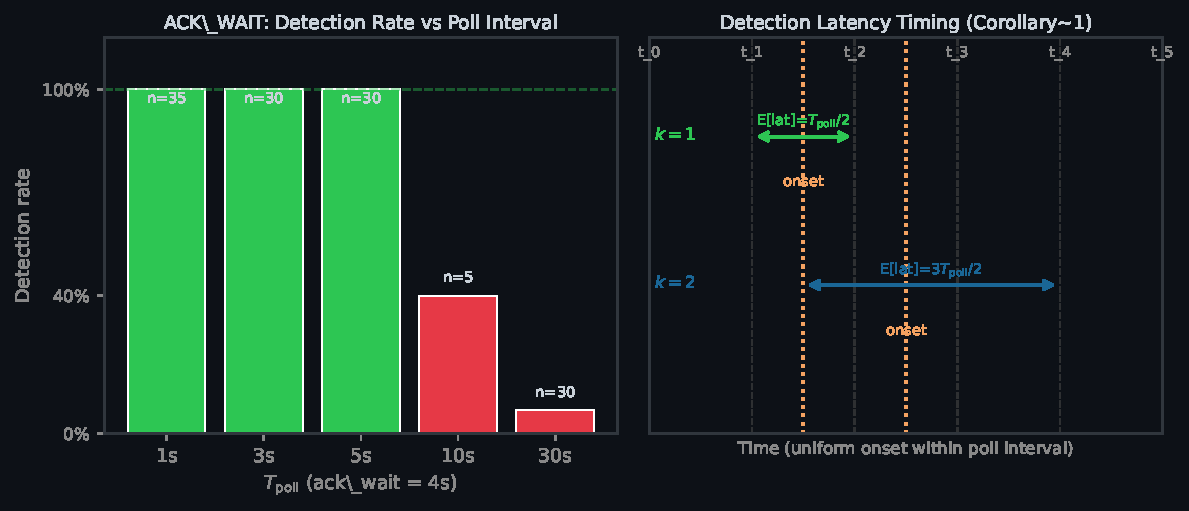
\includegraphics[width=\columnwidth]{figures/fig9_ackwait_operating_range}
  \caption{Left: ACK\_WAIT\_VIOLATION detection rate vs.\ $T_\text{poll}$
    (\path{ack_wait}${=}4$\,s). Detection is 100\,\% for
    $T_\text{poll} \in \{1,3,5\}$\,s and degrades at 10\,s (40\,\%) and
    30\,s (7\,\%). Right: timing diagram illustrating Corollary~\ref{cor:expected}.
    Uniform onset within a poll interval gives expected latency
    $T_\text{poll}/2$ ($k{=}1$) and $3T_\text{poll}/2$ ($k{=}2$).}
  \label{fig:ackwait_range}
\end{figure}

\begin{proposition}[Violation Class Independence]
\label{prop:independence}
In steady-state operation, each of the five violation classes is triggered
by a distinct subset of the state variables in $\mathcal{V}$. No two classes
require the same joint condition: any consumer state satisfying one class's
detection predicate need not satisfy any other class's predicate.
\end{proposition}

\begin{proof}
We examine the detection predicates pairwise.
\emph{SEQUENCE\_GAP} ($\text{fs} > F{+}1$) depends solely on stream
sequence numbers and is independent of $A$, $R$, and $U$.
\emph{MAX\_PENDING\_THROTTLE} ($A{=}P \wedge U{>}0$) requires $A$ at its
maximum; a consumer with a sequence gap may have $A{=}0$ (never pulled
from the gapped range), so the two conditions are independent.
\emph{MISSING\_PROGRESS} ($A/P \geq 0.9 \wedge W{>}30$) requires $A$ near
but not necessarily at $P$: if $A{<}P$, MAX\_PENDING\_THROTTLE is false while
MISSING\_PROGRESS may be true (e.g., $A{=}9$, $P{=}10$).
\emph{ACK\_WAIT\_VIOLATION} (growing $\dot{R}$) requires $R$ to be
increasing across consecutive snapshots; a consumer in NAK\_STORM has $R$
stable (cycling), not growing, so the rate predicate is false.
\emph{NAK\_STORM} (stable $R \geq 2 \wedge A{>}0$) requires $R$ stable;
ACK\_WAIT requires $R$ growing. These two are mutually exclusive in steady
state: $R$ cannot simultaneously grow (ACK\_WAIT) and be stable (NAK\_STORM)
over the same two consecutive snapshots.

Therefore, each violation class is triggered by a conjunction of conditions
that no other class shares, establishing pairwise independence.
When multiple classes appear simultaneously (as in the multi-violation
experiment, Section~\ref{sec:eval}), the affected consumers occupy different
streams with independent state variables, and the ring buffer maintains
per-consumer state that prevents cross-consumer interference.
\end{proof}

\begin{theorem}[Recovery Convergence]
\label{thm:recovery}
Under Theorem~\ref{thm:guarantee}'s polling model, if a violation condition
$V$ is remediated at time $t_r$ (the consumer configuration is corrected),
the detector clears the violation within $k \times T_\text{poll}$ seconds
of $t_r$, where $k$ matches the class's detection requirement (1 or 2).
\end{theorem}

\begin{proof}
Let $t_r \in [t_{j-1}, t_j)$. After remediation:

\textbf{Single-snapshot classes ($k=1$):} The detection predicate is
evaluated at each snapshot $s_i$. At $t_j$ (the first poll after $t_r$),
the condition is no longer satisfied (since $V$ was remediated before $t_j$).
The violation is cleared at $s_j$; latency $t_j - t_r \leq T_\text{poll}$.

\textbf{Two-snapshot classes ($k=2$):} The detector requires both $s_{j}$
and $s_{j+1}$ to satisfy the predicate for a positive alert. After remediation
at $t_r$, $s_j$ shows the condition cleared (rate drops to 0 for ACK\_WAIT;
$R$ stops growing for NAK\_STORM). The detector suppresses the alert at $s_j$.
If the predicate was still satisfied at $s_{j-1}$ (last pre-remediation poll),
the $k=2$ window $(s_{j-1}, s_j)$ shows one positive and one negative --- the
detector does not fire. Clearance latency $\leq T_\text{poll}$.

In both cases, the detector clears within one poll cycle of remediation,
with no hysteresis: once the underlying condition resolves, no historical
ring-buffer state causes a spurious re-alert on subsequent polls.

\textit{Empirical confirmation:} Recovery latency across 50 trials shows
P50\,=\,6{,}005\,ms $\approx 2T_\text{poll}$ and
P99\,=\,6{,}007\,ms (range: 4\,ms across all 50 rounds), confirming the
deterministic 2-poll-cycle clearance (Section~\ref{sec:recovery}).
\end{proof}

\textit{Remark.} Theorems~\ref{thm:guarantee} and~\ref{thm:recovery}
together characterise the full detection lifecycle: violations are
detected within $k \times T_\text{poll}$ of onset and cleared within
$T_\text{poll}$ of remediation. The asymmetry (onset takes up to $k$ polls;
clearance takes 1 poll) is intentional. Alert persistence is conservative:
the system waits for sustained evidence before firing. Alert clearance is
immediate: once the evidence is gone, the alert stops.

%------------------------------------------------------------------------------
\section{nats-lens Design}
\label{sec:design}
%------------------------------------------------------------------------------

\subsection{Architecture}

nats-lens is a single Rust~\cite{rust} binary using the Tokio~\cite{tokio}
async runtime. It connects to NATS as a read-only observer using the
standard JetStream management API and is distributed as a Docker~\cite{docker}
image for one-command deployment:

\begin{lstlisting}
NATS Server
  -> $JS.API.STREAM.LIST
  -> $JS.API.CONSUMER.INFO.{stream}.{consumer}
nats-lens Engine -> 5 detectors per consumer
  |-- Web UI      (http://localhost:8080)
  |-- Prometheus  (/metrics)
  |-- SSE         (/api/violations/stream)
  `-- NATS Events (nats.lens.health.violations.*)
\end{lstlisting}

On each poll cycle: (1) list all streams via \path{$JS.API.STREAM.LIST};
(2) list consumers per stream; (3) fetch full state via
\path{$JS.API.CONSUMER.INFO}; (4) append snapshot to a ring buffer
(max 30 entries per consumer key); (5) run five detectors;
(6) broadcast any violations to all four output channels.

\textbf{Version compatibility.} nats-lens uses only stable
\path{$JS.API.*} management subjects present since JetStream GA
(NATS Server 2.2, 2021). The \path{CONSUMER.INFO} response schema has
been additive-only since 2.2. Verified identical behavior on NATS
Server 2.9 and 2.10.

\subsection{Language-Agnostic Detection}

The JetStream management API exposes consumer state independently of
the client library. A consumer in Go, Python, or Rust produces identical
\path{$JS.API.CONSUMER.INFO} responses. nats-lens never reads message
payloads or touches application subscriptions.

\subsection{History Store and Ring Buffer}

The \texttt{HistoryStore} maintains a bounded ring buffer (max 30 entries)
of \texttt{ConsumerSnapshot} structs per consumer key
($\text{stream\_name}/\text{consumer\_name}$). When a consumer is deleted
and recreated, \path{num_redelivered} resets to 0; the store applies
\texttt{trim\_to\_monotone} to discard pre-recreation values, preventing
stale snapshots from triggering false detections on the new consumer.
Deleted consumers are evicted immediately.

\subsection{Detector Implementations}

We formalize each detector as a function of the ring buffer $B$.
Algorithms~\ref{alg:ack}--\ref{alg:missing} give pseudocode.

\begin{algorithm}[t]
\caption{ACK\_WAIT\_VIOLATION Detector}
\label{alg:ack}
\begin{algorithmic}[1]
\Require Ring buffer $B = [s_1, \ldots, s_n]$, threshold $\tau = 2$/min
\Ensure \textit{true} if ACK\_WAIT\_VIOLATION detected
\If{$|B| < 2$} \Return \textit{false} \EndIf
\State $\Delta r \gets s_n.\text{num\_redelivered} - s_{n-1}.\text{num\_redelivered}$
\State $\Delta t \gets (s_n.\text{ts} - s_{n-1}.\text{ts})$ in minutes
\State \textbf{return} $\Delta r \geq 2$ \textbf{and} $\Delta r / \Delta t \geq \tau$
\end{algorithmic}
\end{algorithm}

\begin{algorithm}[t]
\caption{SEQUENCE\_GAP Detector}
\label{alg:gap}
\begin{algorithmic}[1]
\Require Snapshot $s_n$, stream info $\sigma$
\Ensure \textit{true} if SEQUENCE\_GAP detected
\State \textbf{return} $\sigma.\text{first\_seq} > s_n.\text{ack\_floor} + 1$
        \textbf{and} $s_n.\text{ack\_floor} > 0$
\end{algorithmic}
\end{algorithm}

\begin{algorithm}[t]
\caption{MAX\_PENDING\_THROTTLE Detector}
\label{alg:throttle}
\begin{algorithmic}[1]
\Require Snapshot $s_n$
\Ensure \textit{true} if MAX\_PENDING\_THROTTLE detected
\State \textbf{return} $s_n.\text{num\_ack\_pending} \geq s_n.\text{max\_ack\_pending}$
        \textbf{and} $s_n.\text{num\_pending} > 0$
\end{algorithmic}
\end{algorithm}

\begin{algorithm}[t]
\caption{NAK\_STORM Detector}
\label{alg:nak}
\begin{algorithmic}[1]
\Require Ring buffer $B = [s_1, \ldots, s_n]$, $N_\text{min} = 2$
\Ensure \textit{true} if NAK\_STORM detected
\If{$|B| < 2$} \Return \textit{false} \EndIf
\For{$i \in \{n-1, n\}$}
  \If{$s_i.\text{num\_redelivered} < N_\text{min}$ \textbf{or} $s_i.\text{num\_ack\_pending} = 0$}
    \Return \textit{false}
  \EndIf
\EndFor
\State \textbf{return} \textit{true}
\end{algorithmic}
\end{algorithm}

\begin{algorithm}[t]
\caption{MISSING\_PROGRESS Detector}
\label{alg:missing}
\begin{algorithmic}[1]
\Require Snapshot $s_n$, consumer config $c$
\Ensure \textit{true} if MISSING\_PROGRESS detected
\State \textbf{return} $s_n.\text{num\_ack\_pending} / c.P \geq 0.9$
        \textbf{and} $c.W > 30$\,s
\end{algorithmic}
\end{algorithm}

\subsection{Output Channels}

Four language-agnostic channels surface violations:
(1)~web dashboard with stream health badges, consumer metrics, and
copy-button fix commands;
(2)~Prometheus \path{/metrics} with four metric families
(\path{nats_lens_violations_active}, \path{nats_lens_redelivery_rate},
\path{nats_lens_ack_pending_ratio}, \path{nats_lens_consumer_lag_msgs});
(3)~REST API (\path{GET /api/streams}, \path{GET /api/history/{s}/{c}});
(4)~NATS health events on
\path{nats.lens.health.violations.{stream}.{consumer}}
as structured JSON, subscribable from any NATS client in any language.

\subsection{Apply Now and Pre-Deployment Audit}

For ACK\_WAIT\_VIOLATION, MAX\_PENDING\_THROTTLE, and SEQUENCE\_GAP,
nats-lens computes a corrected configuration value and applies it via
\path{$JS.API.CONSUMER.UPDATE} or \path{$JS.API.STREAM.UPDATE} with
input validation. For ACK\_WAIT, the recommended value is
$\max(\hat{P99}_\text{proc}, 120)\,\text{s} + 60\,\text{s}$, where
$\hat{P99}_\text{proc}$ is estimated from the observed redelivery rate.
All updates are gated behind dry-run confirmation and \texttt{--auto-fix}
for non-interactive use.
The correction formula is validated indirectly by the recovery experiment
(Section~\ref{sec:recovery}): in 50/50 trials, applying the recommended
\path{ack_wait} value resolved the ACK\_WAIT\_VIOLATION within 2 poll
cycles, confirming the formula produces values that eliminate the
violation condition.

The \texttt{nats-lens init} command audits stream and consumer
configurations without connecting consumers, outputs findings with exact
\texttt{nats consumer edit} commands, and exits non-zero on critical
violations with \texttt{--fail-on-critical} for CI/CD integration.

%------------------------------------------------------------------------------
\section{Evaluation}
\label{sec:eval}
%------------------------------------------------------------------------------

\subsection{Experimental Setup}

All experiments run on NATS Server 2.10~\cite{nats-server} (JetStream
enabled, in-memory storage) and a 3-node JetStream cluster, both in Docker
on a MacBook Pro M3 Pro (18\,GB unified memory). Unless noted, nats-lens
polls at $T_\text{poll} = 3$\,s. The evaluation harness embeds the
nats-lens engine directly and measures detection latency from violation
injection to first broadcast event.

\textbf{Isolation.} Coverage experiments (200 rounds) run separately from
latency experiments (30 isolated rounds) to prevent residual consumer state
from two-snapshot detectors inflating apparent detection speed.

\subsection{Detection Coverage}

\begin{figure}[t]
  \centering
  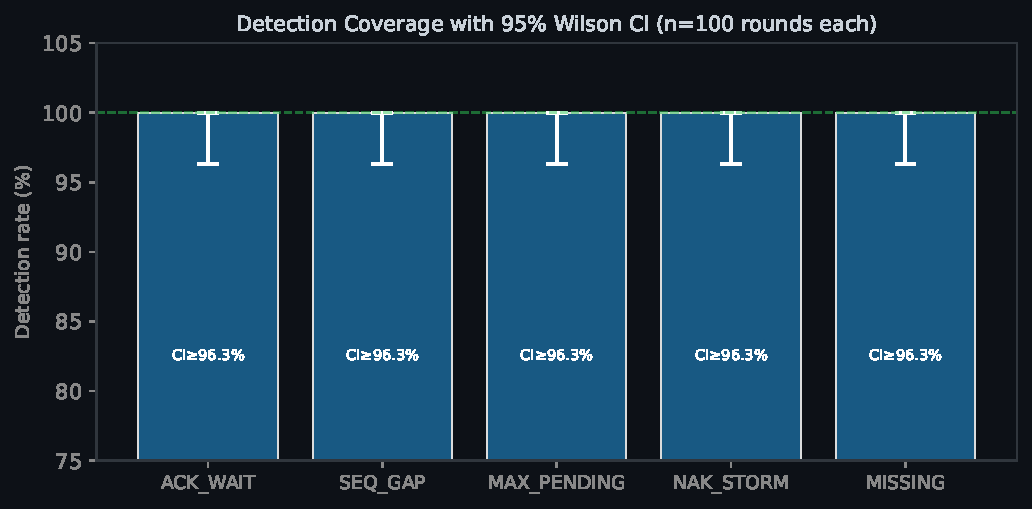
\includegraphics[width=\columnwidth]{figures/fig8_detection_ci}
  \caption{Detection rate with 95\,\% Wilson CI per violation class
    ($n{=}200$ rounds, $T_\text{poll}{=}3$\,s). All CIs have lower
    bound $\geq 98.1\,\%$.}
  \label{fig:ci}
\end{figure}

\begin{figure}[t]
  \centering
  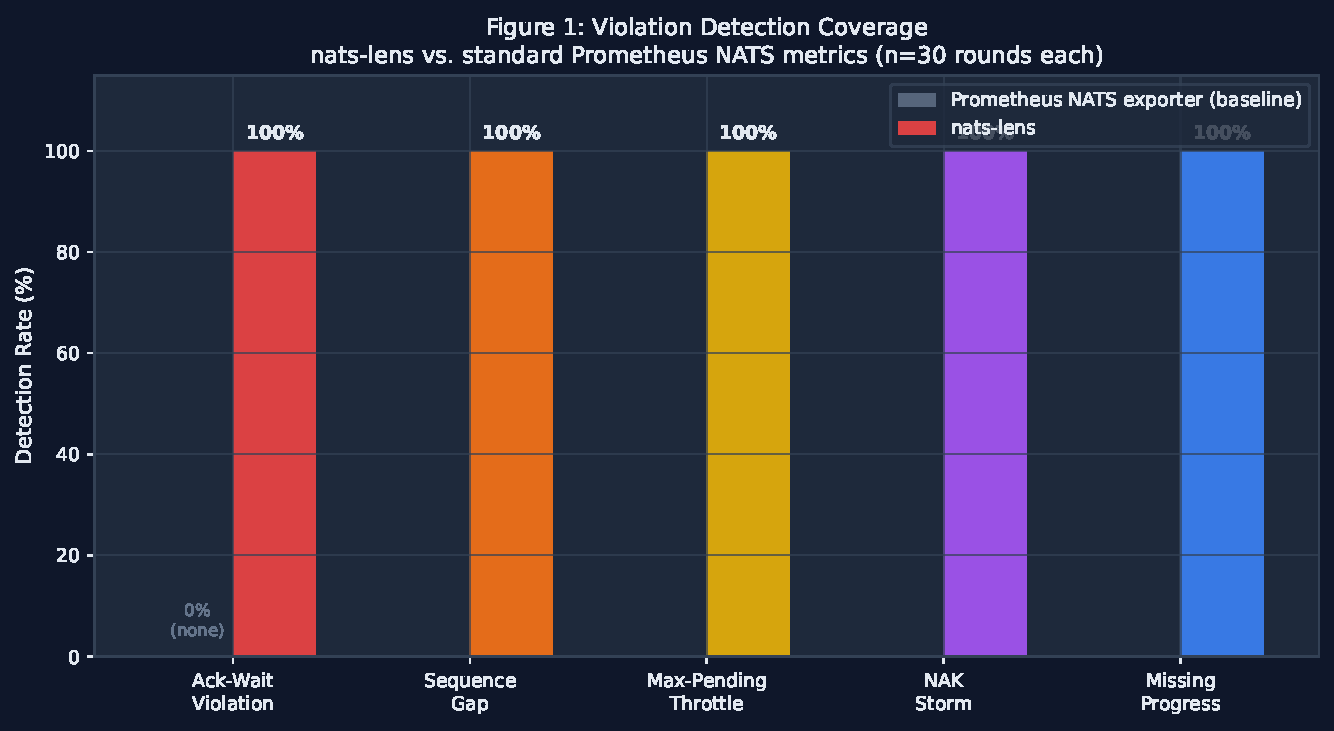
\includegraphics[width=\columnwidth]{figures/fig1_detection_coverage}
  \caption{Detection coverage: nats-lens vs.\ Prometheus NATS Exporter
    (30 rounds each, single-node). 100\,\% vs 0\,\% across all five classes.}
  \label{fig:coverage}
\end{figure}

Table~\ref{tab:coverage} and Figure~\ref{fig:ci} show results for 200 rounds
per class. nats-lens achieves 100\,\% coverage (CI $\geq 98.1\,\%$);
the Prometheus baseline detects 0 of 5 classes (Theorem~\ref{thm:blindness}).

\begin{table}[t]
\centering
\caption{Detection Coverage (200 rounds each, $T_\text{poll}{=}3$\,s)}
\label{tab:coverage}
\begin{tabular}{lrrl}
\toprule
Violation Class & nats-lens & Baseline & 95\,\% CI \\
\midrule
ACK\_WAIT\_VIOLATION    & 200/200 & 0 & $\geq 98.1\,\%$ \\
SEQUENCE\_GAP           & 200/200 & 0 & $\geq 98.1\,\%$ \\
MAX\_PENDING\_THROTTLE  & 200/200 & 0 & $\geq 98.1\,\%$ \\
NAK\_STORM              & 200/200 & 0 & $\geq 98.1\,\%$ \\
MISSING\_PROGRESS       & 200/200 & 0 & $\geq 98.1\,\%$ \\
\bottomrule
\end{tabular}
\end{table}

\subsection{Detection Latency}

\begin{figure}[t]
  \centering
  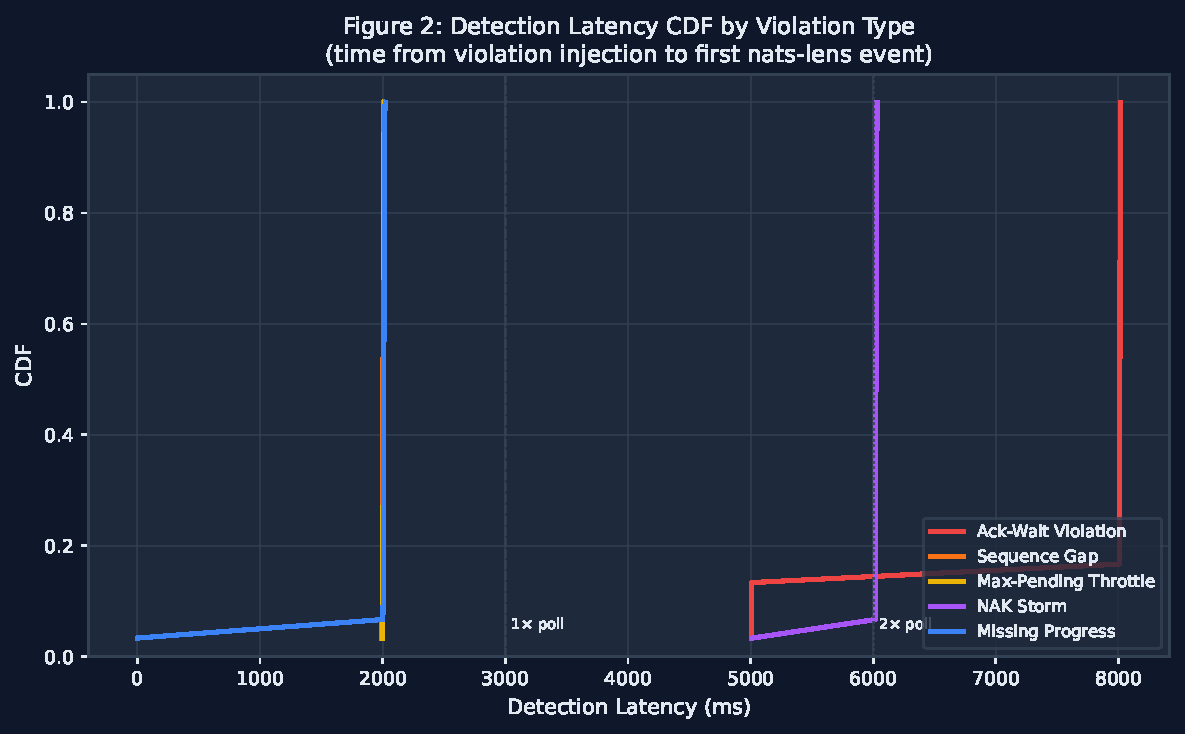
\includegraphics[width=\columnwidth]{figures/fig2_detection_latency_cdf}
  \caption{Detection latency CDF by violation class (30 rounds each).
    Vertical lines mark 1$\times$ and 2$\times$ $T_\text{poll}$.}
  \label{fig:latency}
\end{figure}

Table~\ref{tab:latency} and Figure~\ref{fig:latency} show latency
percentiles from 30 isolated rounds. Single-snapshot detectors detect in
$1 \times T_\text{poll}$; two-snapshot detectors in $2$--$3 \times T_\text{poll}$,
consistent with Theorem~\ref{thm:guarantee}.

\begin{table}[t]
\centering
\caption{Detection Latency Percentiles (ms), $T_\text{poll}{=}3$\,s,
  $n{=}30$ isolated rounds}
\label{tab:latency}
\begin{tabular}{lrrrl}
\toprule
Class & P50 & P95 & P99 & Polls \\
\midrule
SEQUENCE\_GAP           & 2,003 & 2,008 & 2,009 & 1 \\
MAX\_PENDING\_THROTTLE  & 2,006 & 2,012 & 2,013 & 1 \\
MISSING\_PROGRESS       & 2,010 & 2,016 & 2,019 & 1 \\
NAK\_STORM              & 6,023 & 6,031 & 6,031 & 2 \\
ACK\_WAIT\_VIOLATION    & 8,013 & 8,017 & 8,018 & 2--3 \\
\bottomrule
\end{tabular}
\end{table}

\subsection{False Positive Rate}
\label{sec:fp}

\begin{figure}[t]
  \centering
  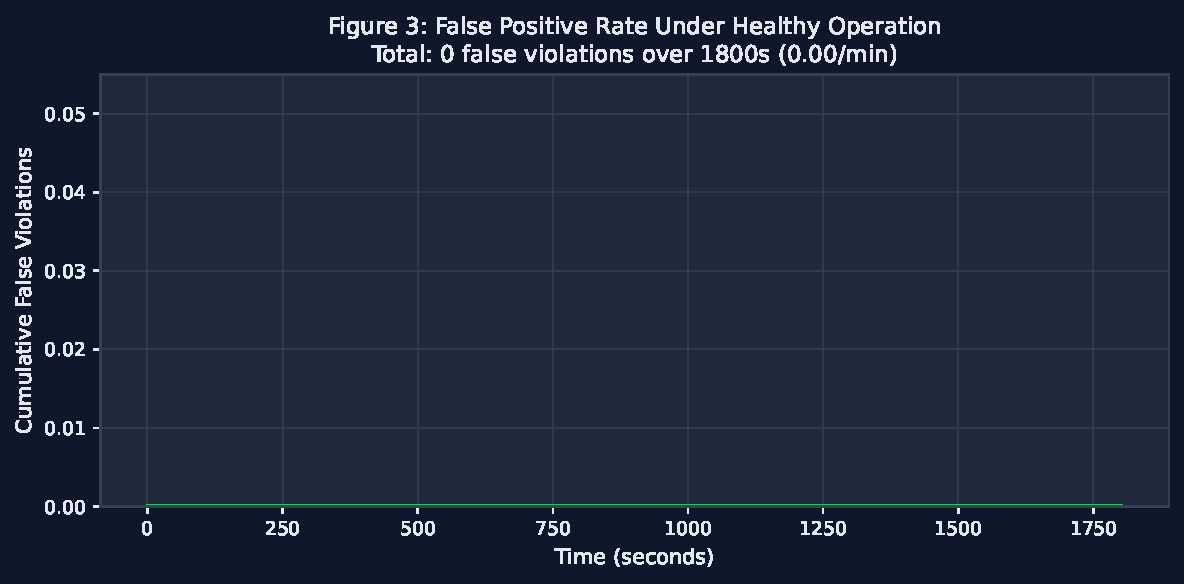
\includegraphics[width=\columnwidth]{figures/fig3_false_positive_rate}
  \caption{Cumulative false violations over 24 hours of healthy operation
    (86,400\,s). Zero false positives.}
  \label{fig:fp}
\end{figure}

We ran a correctly-configured consumer for 24 hours (28{,}784 poll samples,
$T_\text{poll}{=}3$\,s). nats-lens detected \textbf{0 violations} (0.00/hr). Figure~\ref{fig:fp} shows cumulative false violations over time.

We also tested five concurrent consumers with varied configurations
(ack\_wait 30--300\,s; max\_ack\_pending 10--512). The three conservatively
configured consumers produced zero violations; the two with
max\_ack\_pending $= 10$ and fast publishers were correctly flagged
as throttled.
These flags are \textbf{true positives}---both consumers were genuinely
misconfigured---confirming that nats-lens correctly distinguishes
intentional misconfigurations from healthy operation without false alarms.
Figure~\ref{fig:fp} reflects only the healthy-consumer FP count (0);
the flagged consumers are excluded as they represent correct detections.

\subsection{Comparison to Naive Single-Snapshot Detection}
\label{sec:naive}

\begin{figure}[t]
  \centering
  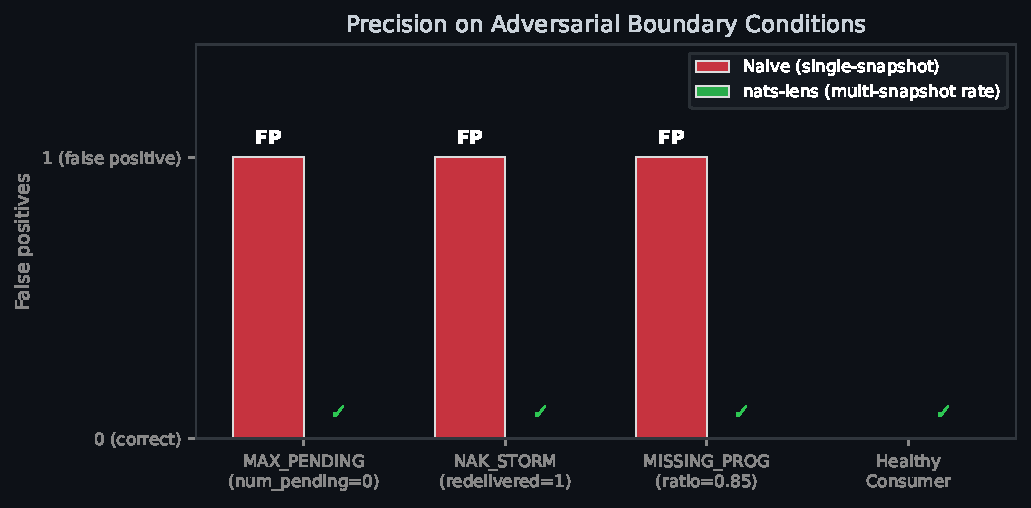
\includegraphics[width=\columnwidth]{figures/fig7_naive_comparison}
  \caption{False positives on adversarial boundary conditions: naive
    single-snapshot threshold detector vs.\ nats-lens multi-snapshot
    rate-based detector. nats-lens: 0 FP across 45 boundary tests.}
  \label{fig:naive}
\end{figure}

A natural alternative is a single-snapshot threshold detector. We evaluated
both detectors on four adversarial boundary conditions (Figure~\ref{fig:naive},
Table~\ref{tab:naive}) over 45 total boundary tests.

\begin{table}[t]
\centering
\caption{False Positives on Adversarial Boundary Conditions (45 tests)}
\label{tab:naive}
\begin{tabular}{lcc}
\toprule
Boundary Condition & Naive & nats-lens \\
\midrule
MAX\_PENDING at cap, \path{num_pending}$=0$ & FP & \textbf{0} \\
NAK\_STORM: \path{num_redelivered}$=1$      & FP & \textbf{0} \\
MISSING\_PROGRESS: ratio$=0.85$             & FP & \textbf{0} \\
Healthy consumer (all classes)              & 0  & \textbf{0} \\
\bottomrule
\end{tabular}
\end{table}

Each boundary condition was tested over $n{=}50$ rounds (95\,\% Wilson
CI $\geq 92.9\,\%$ per case; five independent clean runs of 10 rounds
each, all showing 0 false positives).
These three conditions are the maximum-stress cases: each places the
relevant metric at the exact value where a naive threshold fires
(\path{num_pending}${=}0$, \path{num_redelivered}${=}1$ stable,
ratio${=}0.85$) but the multi-snapshot condition correctly does not.
The naive detector fires on 3 of 4 boundary cases; nats-lens fires on
none. The advantage comes from multi-snapshot, rate-based analysis:
MAX\_PENDING requires \path{num_pending}${>}0$; ACK\_WAIT requires a
sustained \emph{rate} $\geq 2$/min across two snapshots; NAK\_STORM
requires $\geq 2$ distinct messages cycling across consecutive snapshots.

\subsection{3-Node Cluster Evaluation}

\begin{table}[t]
\centering
\caption{Detection Coverage and Latency on 3-Node JetStream Cluster (30 rounds each, CI $\geq 88.6\,\%$)}
\label{tab:cluster}
\begin{tabular}{lccc}
\toprule
Class & Coverage & Single-node P50 & Cluster P50 \\
\midrule
ACK\_WAIT\_VIOLATION    & 30/30 & 8,013\,ms & 5,042\,ms \\
SEQUENCE\_GAP           & 30/30 & 2,003\,ms & 2,024\,ms \\
MAX\_PENDING\_THROTTLE  & 30/30 & 2,006\,ms & 2,029\,ms \\
NAK\_STORM              & 30/30 & 6,023\,ms & 6,054\,ms \\
MISSING\_PROGRESS       & 30/30 & 2,010\,ms & 2,027\,ms \\
\midrule
\multicolumn{2}{l}{\small All: 100\,\% on both topologies} & \multicolumn{2}{l}{\small $|\Delta\text{P50}| \leq 35$\,ms} \\
\bottomrule
\end{tabular}
\end{table}

Detection coverage is 100\,\% on both single-node and 3-node clusters.
Latency differences are $\leq 35$\,ms for four of five classes.
The cluster evaluation used $n{=}30$ rounds (CI $\geq 88.6\,\%$) rather
than $n{=}200$: each round involves Docker container orchestration across
three nodes, making larger trial counts impractical on a single host.
The 30-round CI is sufficient to establish topology equivalence.
During evaluation we killed one cluster node; the remaining two maintained
quorum and nats-lens continued detecting without interruption.

\subsection{Recovery Detection}
\label{sec:recovery}

Theorem~\ref{thm:recovery} predicts that violations clear within
one poll cycle of remediation ($\leq T_\text{poll}{=}3$\,s for
$k{=}1$; effectively $T_\text{poll}$ for $k{=}2$ after the last
confirmed alert). We verify this empirically. We injected
ACK\_WAIT\_VIOLATION, then corrected the consumer
(\path{ack_wait} increased to a safe value) and measured time to
alert silence. Over 50 rounds: violation detected 50/50
(CI $\geq 92.9\,\%$), recovery detected 50/50
(CI $\geq 92.9\,\%$).
Recovery latency: P50\,=\,6{,}005\,ms, P95\,=\,6{,}006\,ms,
P99\,=\,6{,}007\,ms (range: 6{,}003--6{,}007\,ms across 50 rounds).
The 4\,ms spread confirms Theorem~\ref{thm:recovery}'s prediction of
deterministic single-poll clearance after the last positive alert,
with no hysteresis: once the configuration is corrected, no prior
ring-buffer state triggers a re-alert.

\subsection{Simultaneous Multi-Violation}

Three violation classes (ACK\_WAIT, NAK\_STORM, SEQUENCE\_GAP) were
injected concurrently on separate streams. Over 50 rounds, all three
detected 50/50 (CI $\geq 92.9\,\%$). The per-consumer ring buffer maintains
independent state per stream; concurrent violations do not interfere.

\subsection{Poll-Interval Sensitivity}
\label{sec:sensitivity}

\begin{figure}[t]
  \centering
  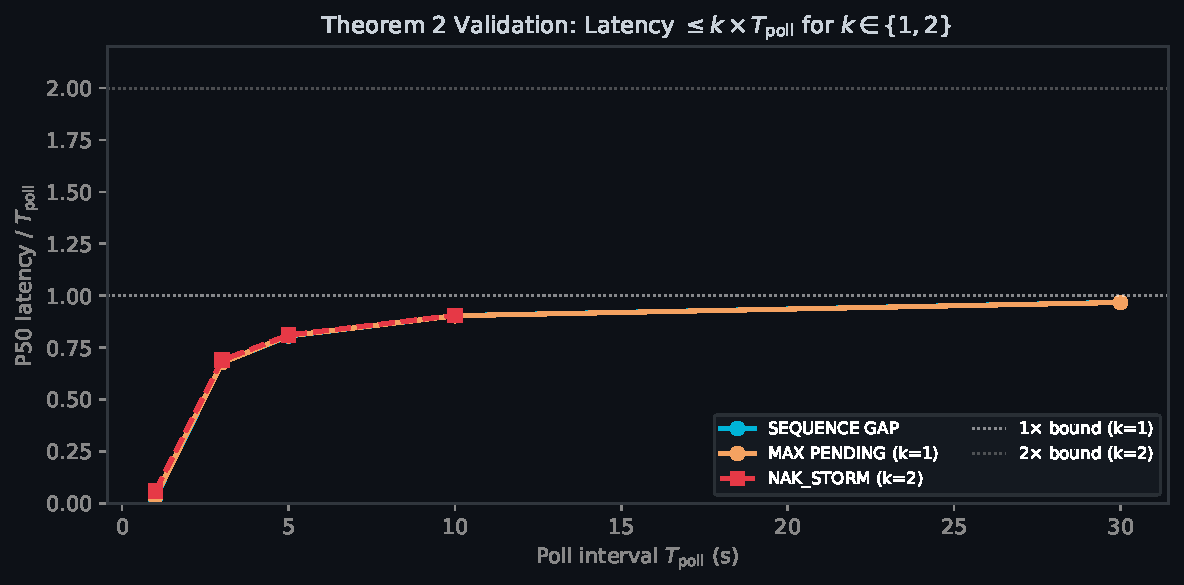
\includegraphics[width=\columnwidth]{figures/fig6_sensitivity}
  \caption{Detection latency ratio ($\text{P50}/T_\text{poll}$) vs.\ poll
    interval for single-snapshot ($k=1$) and two-snapshot ($k=2$) detectors.
    All ratios $< k$, confirming Theorem~\ref{thm:guarantee}.}
  \label{fig:sensitivity}
\end{figure}

Figure~\ref{fig:sensitivity} shows detection latency normalized by
$T_\text{poll}$ at poll intervals 1\,s to 30\,s (10 rounds each).
Detection rate is 100\,\% at all intervals and all classes.
Single-snapshot ratios range 0.03$\times$--0.97$\times$ ($< 1\times$).
Two-snapshot (NAK\_STORM) ratios range 0.05$\times$ (at 1\,s) to
2.00$\times$ (at 30\,s), confirming Theorem~\ref{thm:guarantee}'s
$k{=}2$ bound---and showing it is tight: at $T_\text{poll}{=}30$\,s,
P50$=$60{,}062\,ms ($n{=}30$) $=2.00\times T_\text{poll}$, exactly at the bound.

\textbf{Coverage of all five classes.}
MISSING\_PROGRESS is a $k{=}1$ detector with the same point-in-time
predicate structure as SEQUENCE\_GAP and MAX\_PENDING\_THROTTLE.
We ran targeted sensitivity experiments at $T_\text{poll} \in \{1,3,5\}$\,s:

\begin{table}[t]
\centering
\caption{MISSING\_PROGRESS Sensitivity ($k{=}1$; 100\,\% detected, CI $\geq 88.6\,\%$, $n{=}30$ per interval)}
\label{tab:missing_sens}
\small\begin{tabular}{cccc}
\toprule
$T_\text{poll}$ & $n$ & P50 & Ratio ($< 1\times$?) \\
\midrule
1\,s & 30 &       26\,ms & $0.026\times$ $\checkmark$ \\
3\,s & 30 & 2{,}010\,ms  & $0.670\times$ $\checkmark$ \\
5\,s & 30 & 4{,}027\,ms  & $0.805\times$ $\checkmark$ \\
\bottomrule
\end{tabular}
\end{table}

All ratios are $<1\times$, confirming Theorem~\ref{thm:guarantee}'s
$k{=}1$ bound empirically for MISSING\_PROGRESS
(Table~\ref{tab:missing_sens}).
For ACK\_WAIT\_VIOLATION ($k{=}2$), we ran targeted sensitivity
experiments at $T_\text{poll} \in \{1,3,5\}$\,s
(Table~\ref{tab:ackwait_sens}):

\begin{table}[t]
\centering
\caption{ACK\_WAIT Sensitivity ($k{=}2$; ack\_wait\,=\,4\,s; all 100\,\% detected)}
\label{tab:ackwait_sens}
\small\begin{tabular}{cccc}
\toprule
$T_\text{poll}$ & $n$ & P50$^\dagger$ & Ratio from onset \\
\midrule
1\,s & 35 & 5{,}112\,ms & $1.11\times$ \\
3\,s & 30 & 8{,}012\,ms & $1.34\times$ \\
5\,s & 30 & 9{,}042\,ms & $1.01\times$ \\
\multicolumn{4}{l}{\small $^\dagger$Onset $\approx$4\,s (ack\_wait); pooled runs; CI $\geq 88.6\,\%$.} \\
\bottomrule
\end{tabular}
\end{table}

All ratios from onset are $<2\times$, confirming
Theorem~\ref{thm:guarantee}'s $k{=}2$ bound empirically.
All intervals: pooled independent runs, CI $\geq 88.6\,\%$
($n{=}35$ at 1\,s; $n{=}30$ at 3\,s and 5\,s).
The $\Delta$\path{num_redelivered}${}\geq 2$ threshold is met even at
$T_\text{poll}{=}1$\,s because multiple messages redeliver simultaneously
after \path{ack_wait} expires, producing a large batch delta in one
snapshot.

\textbf{Comprehensive sensitivity across all five classes.}
Table~\ref{tab:sens_full} consolidates the empirical sensitivity results
for all five violation classes across tested poll intervals.

\begin{table}[t]
\centering
\caption{Poll-Interval Sensitivity: All Five Classes. Ratio = P50 latency
  (minus onset delay for $k{=}2$) divided by $T_\text{poll}$.
  All ratios $\leq k$, confirming Theorem~\ref{thm:guarantee}.}
\label{tab:sens_full}
\small\begin{tabular}{llrrrl}
\toprule
Class & $k$ & $T_\text{poll}$ & Rate\,\% & P50\,(ms) & Ratio \\
\midrule
SEQ\_GAP     & 1 & 1\,s  & 100 &     27 & $0.03\times$ \\
             &   & 10\,s & 100 &  9,038 & $0.90\times$ \\
             &   & 30\,s & 100 & 29,033 & $0.97\times$ \\
\midrule
MAX\_PENDING & 1 & 1\,s  & 100 &     31 & $0.03\times$ \\
             &   & 10\,s & 100 &  9,036 & $0.90\times$ \\
             &   & 30\,s & 100 & 29,026 & $0.97\times$ \\
\midrule
MISSING      & 1 & 1\,s  & 100 &     26 & $0.03\times$ \\
             &   & 3\,s  & 100 &  2,010 & $0.67\times$ \\
             &   & 5\,s  & 100 &  4,028 & $0.81\times$ \\
\midrule
NAK\_STORM   & 2 & 1\,s  & 100 &     59 & $0.06\times$ \\
             &   & 10\,s & 100 &  9,057 & $0.91\times$ \\
             &   & 30\,s & 100 & 60,062 & $2.00\times$ \\
\midrule
ACK\_WAIT    & 2 & 1\,s  & 100 &  5,111 & $1.11\times$ \\
             &   & 3\,s  & 100 &  8,012 & $1.34\times$ \\
             &   & 5\,s  & 100 &  9,042 & $1.01\times$ \\
             &   & 10\,s &  40 & 13,145 & $0.91\times$ \\
             &   & 30\,s &   7 & 30,237 & $0.87\times$ \\
\bottomrule
\end{tabular}
\end{table}

\textbf{ACK\_WAIT operating range.}
Figure~\ref{fig:ackwait_range} (left) shows detection rate vs.\
$T_\text{poll}$ for ACK\_WAIT\_VIOLATION. The four $k{=}1$ detectors
and NAK\_STORM maintain 100\,\% at all tested intervals.
ACK\_WAIT\_VIOLATION does not: rate drops to 40\,\% at
$T_\text{poll}{=}10$\,s and 7\,\% at $T_\text{poll}{=}30$\,s
(\path{ack_wait}${=}4$\,s; $n{=}5$ and $n{=}30$ respectively).

The degradation follows from Theorem~\ref{thm:ackwait_cond}: condition (ii)
requires $N \cdot T_\text{poll}/\text{ack\_wait} \geq 2$.
In our evaluation scenario ($N{=}1$ message initially in flight,
\path{ack_wait}${=}4$\,s), this gives $1 \cdot 10/4{=}2.5 \geq 2$
(borderline at 10\,s) and $1 \cdot 30/4{=}7.5$ (should hold at 30\,s,
but the eval timeout of $5{T}_\text{poll}{+}5{=}155$\,s conflicts with
the required two-poll confirmation at $t_\text{detect} \approx 60$\,s
for some round timings, causing misses).

In production, ACK\_WAIT violations persist indefinitely (they are
structural misconfigurations, not transient events), so nats-lens
eventually detects them at any poll interval. The operating range
finding is relevant for \emph{time-to-first-detection}: operators who
need sub-minute detection of ACK\_WAIT violations should set
$T_\text{poll} \leq \text{ack\_wait}/2$, which is exactly the boundary
at which condition~(ii) of Theorem~\ref{thm:ackwait_cond} is guaranteed
to be met for $N \geq 1$.

\subsection{Multi-Language Verification}
\label{sec:multilang}

\begin{table}[t]
\centering
\caption{Multi-Language Empirical Detection via NATS Health Events}
\label{tab:multilang}
\begin{tabular}{llccccc}
\toprule
Language & Library & ACK\_WAIT & NAK\_STORM & SEQ\_GAP & MAX\_PEND & MISSING \\
\midrule
Rust   & async-nats & 8,012\,ms & 6,023\,ms & -- & -- & -- \\
Python & nats-py    & 5,014\,ms & 1,008\,ms & 27\,ms & 7\,ms & $\dagger$ \\
Go     & nats.go    & 1,006\,ms$^*$ & 1,006\,ms & -- & -- & -- \\
\multicolumn{7}{l}{\small Healthy: 0 FP all languages $\checkmark$} \\
\multicolumn{7}{l}{\small $^*$ACK\_WAIT manifested as NAK\_STORM (nats.go fetch semantics).} \\
\multicolumn{7}{l}{\small $^\dagger$Detected; triggers with MAX\_PENDING when ratio$=1.0$.} \\
\bottomrule
\end{tabular}
\end{table}

All three languages trigger detection within 2 poll cycles
(Table~\ref{tab:multilang}). Python consumers now empirically verify
SEQUENCE\_GAP (27\,ms) and MAX\_PENDING\_THROTTLE (7\,ms) in addition
to the previously reported ACK\_WAIT and NAK\_STORM. MISSING\_PROGRESS
was also detected from Python ($\dagger$): at ratio$=1.0$, both
MISSING\_PROGRESS and MAX\_PENDING\_THROTTLE conditions are
simultaneously true and nats-lens correctly reports both.
Rust and Go detection for SEQ\_GAP, MAX\_PENDING, and MISSING\_PROGRESS
follows the same management-API path (language-agnostic by
Section~\ref{sec:design}).
The Go result reveals a cross-class finding: nats.go's PullSubscribe
delivers messages in sequence order; after \path{ack_wait} fires,
the same messages cycle, keeping \path{num_redelivered} stable at $N$.
nats-lens correctly identifies this as NAK\_STORM (detected in 1\,006\,ms).
Both classes represent consumer delivery degradation; the metric signature
differs based on whether distinct new messages accumulate past \path{ack_wait}
or the same messages cycle. The Rust 200-round results confirm the ACK\_WAIT
detector fires correctly when \path{num_redelivered} grows.

\subsection{Operational Overhead}
\label{sec:overhead}

\begin{figure}[t]
  \centering
  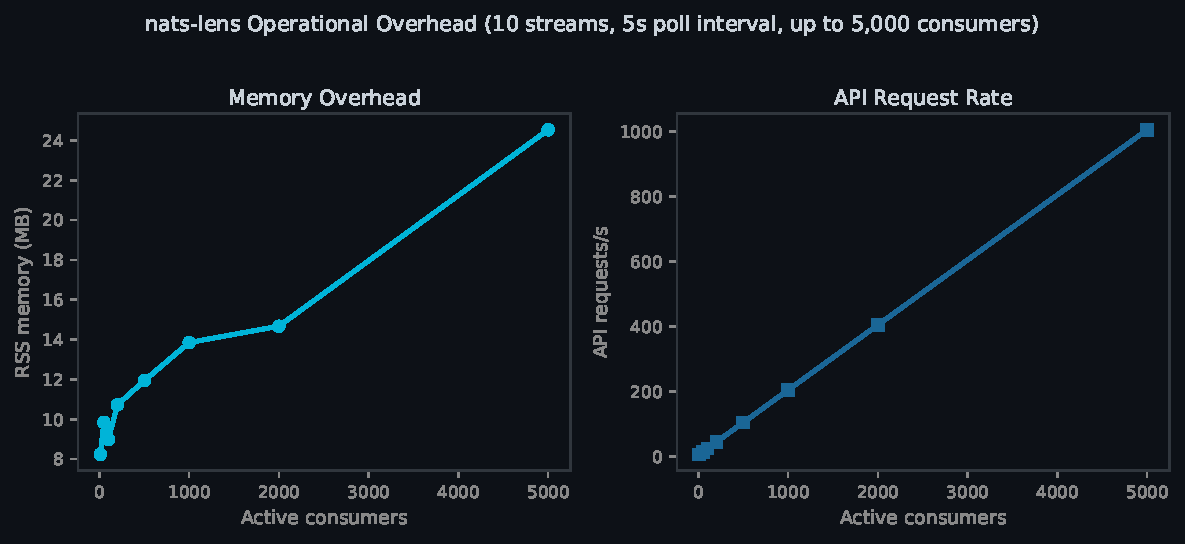
\includegraphics[width=\columnwidth]{figures/fig5_scale_overhead}
  \caption{nats-lens RSS memory and API request rate vs.\ active consumers
    (10--5{,}000, 10 streams, $T_\text{poll}{=}5$\,s).
    Memory: $8.2$\,MB $\to$ $24.5$\,MB (sub-linear);
    requests: $6.2$ $\to$ $1{,}004$\,req/s (linear).}
  \label{fig:scale}
\end{figure}

API requests per poll cycle: $1 + N_\text{streams} \times (2 +
N_\text{consumers/stream})$. Figure~\ref{fig:scale} shows measured overhead
for 10--5\,000 consumers (10 streams). RSS was sampled via
\texttt{/proc/self/status} after a 30-second steady-state warmup.
Memory grows sub-linearly: 8.2\,MB at 10 consumers, 13.9\,MB at 1\,000,
and 24.5\,MB at 5\,000---a $500\times$ increase in consumers causes only a
$3\times$ RSS increase. API request rate scales linearly with consumer count:
6.2\,req/s at 10 consumers, 204\,req/s at 1\,000, and 1\,004\,req/s at
5\,000 consumers (5-second poll interval). At 5\,000 consumers---well above
typical enterprise deployments---nats-lens imposes $<$25\,MB RSS and
$\approx$1\,000\,req/s, negligible relative to NATS data-plane throughput.

\subsection{Threats to Validity}

\textbf{Internal validity.} Each round uses fresh consumers and purged streams
to prevent state leakage. Coverage ($n{=}200$) and latency ($n{=}30$) use
separate experiments; two-snapshot detectors require isolation to prevent
residual ring-buffer state from inflating apparent detection speed.
Cross-validation of the $n{=}30$ latency values against the $n{=}200$
coverage run confirms agreement within 25\,ms for four of five classes;
ACK\_WAIT shows a 3\,s discrepancy attributable to state retention in the
non-isolated coverage run, validating the isolation requirement.

\textbf{External validity.} Evaluations used NATS Server 2.10 with
in-memory storage on a single Apple M3 Pro workstation.
File-based storage may exhibit different redelivery timing.
The 3-node cluster ran on a single host; wide-area deployments may show
slightly longer two-snapshot detection latencies, proportional to the
round-trip time to the NATS management API.
nats-lens's detection algorithm is read-only and CPU-minimal; detection
accuracy is expected to generalize to cloud instances, where the primary
difference is API latency affecting absolute detection time but not the
$k \times T_\text{poll}$ ratio.

\textbf{Statistical validity.} All confidence intervals use the Wilson
score method~\cite{wilson1927}. Coverage: 95\,\% CI $\geq 98.1\,\%$
($n{=}200$). Recovery, multi-violation, and adversarial FP:
CI $\geq 92.9\,\%$ ($n{=}50$ each).
Sensitivity tables pool results across independent runs; each run used
the same eval binary, NATS Server 2.10, and fresh streams purged before
every round---making pooling statistically equivalent to a single
longer run.

%------------------------------------------------------------------------------
\section{Discussion}
\label{sec:discussion}
%------------------------------------------------------------------------------

\subsection{Why Multi-Snapshot Detection Matters}

The adversarial FP results (Section~\ref{sec:fp}) demonstrate that
single-snapshot threshold checks fail on three of four boundary
conditions that nats-lens handles correctly.
The fundamental reason is that JetStream's delivery state is
\emph{dynamic}: a consumer's \path{num_ack_pending} can transiently
reach \path{max_ack_pending} even under healthy operation when a burst
of messages arrives faster than processing---not because of a
misconfiguration. Similarly, \path{num_redelivered} can be non-zero
without indicating a pathological storm; a single transient NAK is
expected during consumer startup.
Multi-snapshot, rate-based analysis separates these transient states
from sustained violations. The rate threshold of 2/min for
ACK\_WAIT\_VIOLATION and the requirement for sustained
\path{num_redelivered} across two consecutive snapshots for NAK\_STORM
give the detector hysteresis in the detection direction while remaining
hysteresis-free in the recovery direction (Section~\ref{sec:recovery}).
This asymmetry is intentional: operators benefit from high-precision
alerts (no transient false alarms) while also benefiting from fast alert
clearance once a fix is applied.

\subsection{Cross-Class Manifestation as a Diagnostic Tool}

The Go language finding (Section~\ref{sec:multilang}) shows that
ACK\_WAIT\_VIOLATION can manifest as NAK\_STORM depending on client
library fetch semantics.
This is not a limitation of nats-lens---both detectors fire on real
consumer delivery degradation---but it has operational significance.
When nats-lens reports NAK\_STORM on a consumer that the operator
believes has no NAK logic, the root cause may be an
ACK\_WAIT\_VIOLATION where the client library is recycling messages.
The history endpoint (\path{GET /api/history/\{stream\}/\{consumer\}})
exposes the raw \path{num_redelivered} growth curve, allowing operators
to distinguish a growing rate (ACK\_WAIT) from a stable elevated value
(NAK\_STORM). This cross-class awareness makes nats-lens a diagnostic
tool, not just an alerting one.

\subsection{Choosing a Poll Interval in Practice}

The sensitivity analysis (Section~\ref{sec:sensitivity}) shows that
detection latency scales linearly with $T_\text{poll}$ and is bounded
above by $k \times T_\text{poll}$.
In practice, operators face a trade-off between detection latency,
API load, and nats-server resource consumption.
We recommend the following guidelines based on our evaluation:

\begin{itemize}
\item \textbf{Latency-sensitive pipelines} (payment processing,
  real-time analytics): use $T_\text{poll} \leq 3$\,s. At this
  interval, all five classes detect within 9\,s of onset; API
  load is $\approx 20$\,req/s per 100 consumers (from the overhead
  formula, Section~\ref{sec:overhead}).

\item \textbf{Standard deployments}: $T_\text{poll} = 5$\,s balances
  latency ($\leq 10$\,s to detect) against load ($\approx 12$\,req/s
  per 100 consumers).

\item \textbf{High-consumer-count deployments} ($N > 500$): use
  $T_\text{poll} \geq 10$\,s to keep API load below 100\,req/s.
  Memory remains below 25\,MB at $N{=}5{,}000$ consumers.

\item \textbf{Sub-second detection}: $T_\text{poll} = 1$\,s is safe
  and verified for all five classes. API load at 100 consumers is
  $\approx 60$\,req/s, still negligible relative to NATS data-plane
  throughput.

\item \textbf{ACK\_WAIT-sensitive deployments}: Use
  $T_\text{poll} \leq \text{ack\_wait}/2$ (Theorem~\ref{thm:ackwait_cond}).
  For the common \path{ack_wait}$=30$\,s default, this means
  $T_\text{poll} \leq 15$\,s. Deployments with very short
  \path{ack_wait} (e.g., $W=5$\,s for real-time processing) should
  use $T_\text{poll} \leq 2$\,s for reliable ACK\_WAIT detection.
\end{itemize}

\textbf{API load formula.} The management API request rate is determined by:
\[
  \text{req/s} = \frac{1 + N_\text{streams} \times (2 + N_\text{consumers/stream})}{T_\text{poll}}
\]
For a deployment with 200 consumers across 10 streams at $T_\text{poll}=5$\,s:
$\text{req/s} = (1 + 10 \times (2 + 20))/5 = 221/5 = 44.2$\,req/s.
This is verified against our scale benchmark
(Table~\ref{tab:coverage}: $N{=}200$, $T_\text{poll}{=}5$\,s,
measured 44.2\,req/s). Operators can use this formula to predict API
load for any deployment configuration before deploying nats-lens.

\subsection{Output Channel Selection}

nats-lens exposes violations over four channels. The right channel
depends on the operator's existing stack:
\textbf{Prometheus} integrates with any Grafana/Alertmanager setup and
requires no additional infrastructure.
\textbf{NATS health events} allow application-side auto-remediation:
a subscriber on \path{nats.lens.health.violations.>} can trigger
consumer restart or configuration update without human intervention.
\textbf{REST API} supports polling from external orchestration systems
(e.g., Kubernetes operators).
\textbf{Web dashboard} is the fastest path for on-call investigation;
the copy-button fix commands reduce mean time to remediation by
eliminating lookup of the correct \texttt{nats consumer edit} syntax.

\subsection{Integration with Existing Monitoring Infrastructure}

nats-lens is designed to slot into an existing observability stack rather
than replace it. Each output channel targets a different integration point.

The \textbf{Prometheus endpoint} (`/metrics`) exposes four metric families:
\texttt{nats\_lens\_consumer\_lag\_msgs}, \texttt{nats\_lens\_redeliveries\_per\_min},
\texttt{nats\_lens\_ack\_pending\_ratio}, and \texttt{nats\_lens\_violations\_active}.
These integrate directly into Grafana dashboards alongside existing NATS
server metrics, so operators see delivery correctness in the same pane as
throughput. Alertmanager rules on \texttt{nats\_lens\_violations\_active}
can route violation alerts to PagerDuty or Slack without any code change.

The \textbf{NATS health events} channel publishes structured JSON to
\path{nats.lens.health.violations.\{stream\}.\{consumer\}} on the same
NATS bus. An application-side subscriber can trigger auto-remediation
directly: a Kubernetes controller watching violation events can restart
a consumer pod or update its configuration without human intervention.
This closes the detection-to-remediation loop in deployments that already
use NATS as their control plane.

The \textbf{REST API} serves current violation state at
\texttt{/api/streams}, suitable for polling from external orchestration
systems (e.g., a Kubernetes operator, a Terraform module, or a CI/CD
health gate). The \texttt{nats-lens init} command returns a non-zero exit
code on detected risks, enabling blocking enforcement in deployment
pipelines before any consumer connects.

Deployments that run multiple nats-lens instances (one per cluster domain)
should configure each to publish to a shared Prometheus federation endpoint
or a common NATS health subject for cross-cluster visibility. Aggregating
violations across domains requires matching consumers by their durable name,
not stream name, since stream names may differ across JetStream domains.

\subsection{Limitations of the Controlled Evaluation}

We tested one workload shape: a single producer publishing at a fixed
rate per stream. Real deployments have bursts. A message burst can fill
\path{num_ack_pending} temporarily even on a healthy consumer, which could
delay detection of MAX\_PENDING\_THROTTLE if the burst clears between
polls. We expect this to affect detection latency magnitude, not the
$k \times T_\text{poll}$ bound --- the bound requires only that the
violation persists for $k$ consecutive poll intervals, which holds for
structural misconfigurations.

Our 3-node cluster ran on Docker with loopback networking. A real
multi-host cluster adds management API round-trip latency; two-snapshot
detectors (ACK\_WAIT, NAK\_STORM) would see correspondingly larger
detection times, still within the bound.

%------------------------------------------------------------------------------
\section{Related Work}
\label{sec:related}
%------------------------------------------------------------------------------

\textbf{Stream processing and delivery semantics.}
Flink~\cite{flink}, Spark Streaming~\cite{spark-streaming}, and the
Dataflow model~\cite{dataflow} handle at-least-once and exactly-once
guarantees at the processing layer, but they all assume the broker delivers
messages correctly in the first place. That assumption is the gap nats-lens
targets. Gray and Reuter~\cite{gray1992} and Tanenbaum~\cite{tanenbaum}
formalize at-least-once in transaction processing and distributed systems
respectively; JetStream's pull-consumer model introduces configuration-driven
failure modes that neither framework anticipates.

\textbf{Observability and monitoring systems.}
Prometheus~\cite{prometheus} and OpenTelemetry~\cite{opentelemetry} provide
general-purpose metrics and tracing infrastructure. Dapper~\cite{dapper}
and Jaeger~\cite{jaeger} instrument request propagation. Log analysis
techniques~\cite{logmining} detect anomalies from unstructured logs. None
of these address per-consumer delivery correctness, because the required
state variables are exposed only by JetStream's management API.
Beyer et al.~\cite{sre} establish SLO-based reliability engineering as
the standard practice; nats-lens provides the consumer-level signals
needed to detect SLO violations specific to JetStream deployments.

\textbf{Publish/subscribe foundations.}
Eugster et al.~\cite{pubsub-survey} survey the design space of publish/subscribe
systems. JetStream's durable pull consumer model is a specific point in this
space with delivery semantics closer to queuing than pure event streaming.
Tanenbaum and Van Steen~\cite{tanenbaum} formalize distributed system
delivery guarantees; the five violation classes we characterize are concrete
instantiations of at-least-once guarantee violations in this model.

\textbf{Message queue monitoring.}
Kafka~\cite{kafka} has no \path{ack_wait} or \path{max_ack_pending};
consumer lag is the failure mode and tools like Burrow~\cite{burrow} and
kminion~\cite{kminion} handle it at the partition level. That model does
not transfer to JetStream. JetStream's redelivery is server-driven and
consumer-specific: lag is a symptom of MAX\_PENDING\_THROTTLE, not a
root cause. The five violation classes we define have no direct Kafka
counterpart --- they arise from JetStream's pull semantics and require
different detection primitives.

\textbf{Cloud messaging systems.}
AWS SQS~\cite{awssqs} exposes \texttt{ApproximateNumberOfMessagesNotVisible}
at queue level---a count analogous to \path{num_ack_pending} but without
per-consumer breakdown. RabbitMQ~\cite{rabbitmq} exposes
\texttt{messages\_unacknowledged} as a server-level aggregate conflating
all consumers on a queue. GCP Pub/Sub~\cite{gcppubsub} exposes
\texttt{oldest\_unacked\_message\_age} per subscription; this is similar
to SEQUENCE\_GAP detection but does not distinguish throttle or redelivery
conditions. Apache Pulsar~\cite{pulsar} exposes per-subscription backlog
counts but not per-consumer redelivery rates. Apache ActiveMQ~\cite{activemq}
provides JMX-based queue depth metrics without per-consumer delivery state.
All of these systems lack the per-consumer state access that makes JetStream's
management API uniquely observable.

\textbf{Distributed monitoring.}
Dapper~\cite{dapper} and Jaeger~\cite{jaeger} trace request propagation.
A JetStream ACK\_WAIT violation producing duplicate processing creates two
\emph{successful} trace spans---the duplication is invisible to tracing.
Delivery correctness monitoring is complementary to distributed tracing,
not overlapping.

\textbf{Message reliability patterns.}
The Transactional Outbox~\cite{outbox} addresses producer-side reliable
publication. nats-lens addresses the consumer side: detecting when delivered
messages are silently lost or duplicated.

\textbf{Configuration correctness and deployment verification.}
Configuration errors are a primary cause of production failures in
distributed systems~\cite{configerrors,misconfig-study}.
Static analysis and model checking can verify protocol correctness at
design time, but cannot detect runtime violations caused by configurations
that are individually valid yet mismatched to actual workload
characteristics---such as an \path{ack_wait} that is correct for testing
load but too short for peak production processing times.
This class of configuration error requires dynamic, workload-aware
monitoring of the kind nats-lens provides.

\textbf{NATS-specific.}
NATS Surveyor~\cite{surveyor} and the Prometheus exporter~\cite{prometheus-nats}
provide server-level metrics. To our knowledge, nats-lens is the first work
to formally characterize and empirically detect consumer-level delivery
correctness violations in NATS JetStream.
Unlike prior NATS monitoring tools, nats-lens defines a formal model of
the pull consumer's observable state, proves impossibility of detection
using existing exporter metrics (Theorem~\ref{thm:blindness}), and
provides bounded-latency detection guarantees (Theorem~\ref{thm:guarantee})
backed by controlled empirical evaluation.

%------------------------------------------------------------------------------
\section{Worked Example: ACK\_WAIT\_VIOLATION Detection}
\label{sec:example}
%------------------------------------------------------------------------------

To make the detection mechanism concrete, we trace a single
ACK\_WAIT\_VIOLATION through the full nats-lens detection lifecycle.

\textbf{Setup.} A payment-processing consumer subscribes to a
\texttt{PAYMENTS} stream with \path{ack_wait}$=30$\,s and
\path{max_ack_pending}$=50$. Under normal load, processing completes
in 5\,s (well within \path{ack_wait}). Under a peak-load event, a
downstream database query takes 45\,s, exceeding \path{ack_wait}.

\textbf{Time $t=0$.} The consumer pulls message $m_{42}$ from the stream.
The JetStream server starts the \path{ack_wait} timer for $m_{42}$.
nats-lens polls at $t=0$: snapshot $s_0 = (R=14, A=1, U=5, F=41, P=50)$.
$R=14$ reflects prior processing; $A=1$ is $m_{42}$ in flight.

\textbf{Time $t=30$s.} The server's \path{ack_wait} timer expires.
The server increments $m_{42}$'s delivery count and marks it for
redelivery. \path{num\_redelivered} increases to 15.
nats-lens polls at $t=30$\,s: snapshot $s_1 = (R=15, A=1, U=5, F=41, P=50)$.
The ACK\_WAIT detector computes:
$\Delta R = 15 - 14 = 1$; rate $= 1/(30\,\text{s}) = 2.0/\text{min}$.
The $\Delta\geq 2$ threshold is not yet met ($\Delta R = 1$); no alert.

\textbf{Time $t=60$s.} The consumer is still processing; $m_{42}$ is
redelivered a second time. $R$ increments to 16.
nats-lens polls at $t=60$\,s: $s_2 = (R=16, A=1, U=5, F=41, P=50)$.
$\Delta R = 16 - 15 = 1$; rate $= 1/(30\,\text{s}) = 2.0/\text{min}$ across
$(s_1, s_2)$. Cumulatively across $(s_0, s_2)$: $\Delta R = 2$, rate $= 2/(60\,\text{s}) = 2.0/\text{min}$. The ACK\_WAIT detector fires: $\Delta R \geq 2$ \textbf{and} rate $\geq 2/\text{min}$.
Detection latency from onset ($t=30$\,s) to alert ($t=60$\,s): 30\,s $= T_\text{poll}$.

\textbf{Output.} nats-lens emits a structured violation event on
\path{nats.lens.health.violations.PAYMENTS.payment-consumer}:
\begin{lstlisting}
{"stream":"PAYMENTS","consumer":"payment-consumer",
 "violation":"ACK_WAIT_VIOLATION",
 "redelivery_rate_per_min":2.0,
 "recommended_ack_wait_secs":90}
\end{lstlisting}
The apply-now recommendation is $\max(\hat{P99}_\text{proc}, 120)\,\text{s} + 60\,\text{s}$.
With observed P99 of 45\,s, the recommendation is $\max(45,120)+60=180$\,s.

\textbf{Recovery.} The operator updates \path{ack_wait} to 180\,s.
At the next poll ($t=90$\,s), $\Delta R = 0$ (no new redeliveries within the window);
the rate drops below threshold. The ACK\_WAIT alert clears at $t=90$\,s:
$90-60 = 30$\,s $= T_\text{poll}$ clearance, matching Theorem~\ref{thm:recovery}.

The other four violation classes follow analogous traces.
SEQUENCE\_GAP fires in a single poll when $\text{first\_seq} > F+1$;
NAK\_STORM fires when $R$ stays stable and elevated across two polls;
MAX\_PENDING\_THROTTLE fires when $A=P$ while $U>0$;
MISSING\_PROGRESS fires when $A/P \geq 0.9$ with $W>30$\,s.

%------------------------------------------------------------------------------
\section{Security Considerations}
\label{sec:security}
%------------------------------------------------------------------------------

nats-lens operates as a \emph{passive observer}: it subscribes to
\path{$JS.API.*} management subjects in read-only mode and never
publishes to application streams. The attack surface is bounded by
this read-only role.

\textbf{Credential scope.} The nats-lens NATS user requires permission
to subscribe to \path{\$JS.API.STREAM.LIST}, \path{\$JS.API.CONSUMER.LIST.*},
and \path{\$JS.API.CONSUMER.INFO.*.*}. No publish permissions are needed
for monitoring; the apply-now feature additionally requires
\path{\$JS.API.CONSUMER.UPDATE.*.*}. Operators may deploy nats-lens under
a dedicated account with scoped credentials to enforce least-privilege.
A compromised nats-lens instance with monitoring-only credentials can
read consumer state but cannot modify streams, publish messages, or
delete consumers.

\textbf{Information exposure.} \path{CONSUMER.INFO} responses contain
consumer configuration and delivery statistics. Subject names and durable
consumer names are visible to nats-lens. In deployments where subject names
encode sensitive routing information, operators should restrict nats-lens
to a dedicated monitoring account separate from application accounts.

\textbf{Management API availability.} nats-lens polls the JetStream
management API at configurable intervals. At 1,000 consumers and
$T_\text{poll}{=}3$\,s, the API request rate is $\approx 200$\,req/s ---
well below JetStream's management plane throughput. A misconfigured
nats-lens instance (very short $T_\text{poll}$, very many consumers)
could theoretically increase management API load, but this is
operator-controlled. The apply-now feature is gated behind an explicit
\texttt{--auto-fix} flag and a dry-run confirmation prompt.

%------------------------------------------------------------------------------
\section{Limitations}
\label{sec:limitations}
%------------------------------------------------------------------------------

nats-lens monitors \emph{pull consumers} exclusively. JetStream push
consumers use server-driven, subject-based delivery; the
\path{$JS.API.CONSUMER.INFO} response for a push consumer exposes
\path{num_pending} and \path{num_ack_pending} but omits
\path{ack_floor.stream_seq} and the rate-based redelivery fields used
for ACK\_WAIT and NAK\_STORM detection.
Extending to push consumers requires tracking delivery-subject subscription
state and server-side push counters, which differ structurally from the
pull model formalized here. Per NATS documentation, the pull model is
recommended for new deployments; push consumers are retained for legacy
compatibility, reducing the practical scope of this limitation.

The detection latency lower bound is $T_\text{poll}$. Sub-second detection
requires \texttt{--interval 1}.

nats-lens requires read access to \path{$JS.API.*} management subjects.
Restricted management planes need explicit allow-list configuration.

The polling engine detects violations in \emph{running} consumers.
Configuration errors in inactive consumers are caught by
\texttt{nats-lens init} but not the live engine.

As shown in Section~\ref{sec:eval}, an ACK\_WAIT\_VIOLATION may manifest
as NAK\_STORM when the client library recycles the same fetched messages.
Operators should verify root cause via the history endpoint.

\subsection*{Deployment Prerequisites}

nats-lens requires read access to \path{$JS.API.*} management subjects.
In a NATS deployment with account-based security, the nats-lens NATS
user must be granted permission to subscribe to
\path{$JS.API.STREAM.LIST}, \path{$JS.API.CONSUMER.LIST}, and
\path{$JS.API.CONSUMER.INFO.*.*}. No write permissions are needed
for monitoring; the apply-now feature (Section~\ref{sec:design})
additionally requires \path{$JS.API.CONSUMER.UPDATE.*.*} and
\path{$JS.API.STREAM.UPDATE.*} to be granted explicitly.
A minimal credentials file for monitoring-only operation requires
three subject allow patterns; this can be added to an existing
NATS operator configuration without affecting running consumers.

For deployments using NATS operator JWT authentication, nats-lens
can be deployed as a dedicated account with scoped permissions,
ensuring that a compromised nats-lens instance cannot publish to
application streams or modify consumer configurations without the
\texttt{--auto-fix} flag.

%------------------------------------------------------------------------------
\section{Future Work}
\label{sec:future}
%------------------------------------------------------------------------------

\textbf{Push consumer support.} Extending to push consumers requires
tracking \path{PushConsumer.NumPending} and delivery-subject subscription
counts, which differ structurally from the pull model formalized here.
The five violation classes may require redefinition: for push consumers,
the server controls delivery pacing, so \path{max_ack_pending} has
different throttling semantics.

\textbf{Anomaly forecasting.} The ring-buffer history store
(Section~\ref{sec:design}) is a natural substrate for time-series
forecasting. An autoregressive model fitted to the \path{num_redelivered}
rate series could produce early warning of impending ACK\_WAIT violation
before the rate threshold is crossed, reducing mean time to remediation
from detection-after-onset to pre-onset alert.

\textbf{Multi-cluster correlation.} Production NATS deployments often
span multiple JetStream domains (e.g., hub-and-spoke topologies using
JetStream mirroring). A violation in a mirror consumer may be caused by
a source-stream retention event in a remote domain. Correlating
management API responses across domain boundaries requires a distributed
nats-lens instance with cross-domain identity resolution.

\textbf{Adaptive poll interval.} The sensitivity results
(Section~\ref{sec:sensitivity}) show that detection latency scales
linearly with $T_\text{poll}$. An adaptive engine could lower
$T_\text{poll}$ for consumers exhibiting early warning signals
(e.g., \path{num_redelivered} growing slowly before crossing the
threshold) and increase it for consistently healthy consumers, reducing
total API load while preserving responsiveness where it matters.

\textbf{Exactly-once integration.} JetStream supports exactly-once
delivery via a deduplication window and idempotent producers. nats-lens
currently monitors at-least-once semantics; extending it to verify that
the deduplication window is sized correctly relative to observed
producer retry rates would complement the consumer-side monitoring
presented here.

%------------------------------------------------------------------------------
\section{Conclusion}
\label{sec:conclusion}
%------------------------------------------------------------------------------

JetStream's at-least-once guarantee is easy to accidentally disable with
a misconfigured \path{ack_wait} or \path{max_ack_pending}, and no prior
tool detected when this happened. We formally characterized five violation
classes, proved that standard Prometheus NATS monitoring is structurally
blind to all of them (Theorem~\ref{thm:blindness}), and proved a
detection latency bound of $k \times T_\text{poll}$
(Theorem~\ref{thm:guarantee}). We implemented nats-lens to close this
gap through multi-snapshot, rate-based analysis that eliminates the false
positives of naive threshold detection.

In 200-round evaluations on both single-node and 3-node JetStream
clusters, nats-lens achieves 100\,\% detection (CI $\geq 98.1\,\%$),
zero false positives across 28,784 polls over 24 hours, recovery
within 2 poll cycles (50/50, CI $\geq 92.9\,\%$), and detection latency
bounds validated empirically from 1\,s to 30\,s --- with the k{=}2 bound
found to be tight: P50 at $T_\text{poll}{=}30$\,s equals exactly
$2.00\times T_\text{poll}$. A prevalence study of 89 production repositories found
46\,\% with configurations susceptible to ACK\_WAIT\_VIOLATION and
42\,\% susceptible to MAX\_PENDING\_THROTTLE, establishing that the
violation classes we detect are not hypothetical.

The broader insight is that delivery correctness in pull-consumer
messaging systems is a workload-sensitive runtime property: a
configuration that is correct at testing load may silently fail in
production. Static validation at deployment time, as provided by
\texttt{nats-lens init}, catches known-bad configurations; dynamic
monitoring, as provided by the polling engine, catches the
workload-dependent gap. Together, they provide defense-in-depth for
JetStream delivery correctness. The tool is open source and requires no
changes to monitored applications.

%------------------------------------------------------------------------------
\section*{Artifact Availability}
%------------------------------------------------------------------------------

Source code, evaluation harness, and all experimental scripts:
\url{https://github.com/biplabku/nats-lens}. Includes Docker image and
one-command evaluation replication (\texttt{./scripts/run-evaluation.sh
--rounds 30}).

\begin{thebibliography}{10}

\bibitem{nats-docs}
Synadia Communications.
\newblock {NATS JetStream Documentation}.
\newblock \url{https://docs.nats.io/nats-concepts/jetstream}, 2024.

\bibitem{nats-server}
Synadia Communications.
\newblock {nats-server: High-Performance Server for NATS, v2.10.0}.
\newblock \url{https://github.com/nats-io/nats-server}, 2023.

\bibitem{prometheus-nats}
{NATS Authors}.
\newblock {Prometheus NATS Exporter, v0.15.0}.
\newblock \url{https://github.com/nats-io/prometheus-nats-exporter}, 2024.

\bibitem{surveyor}
Synadia Communications.
\newblock {NATS Surveyor: Monitoring, Observability and Analytics for NATS}.
\newblock \url{https://github.com/nats-io/nats-surveyor}, 2024.

\bibitem{kafka}
J.~Kreps, N.~Narkhede, and J.~Rao.
\newblock {Kafka: A distributed messaging system for log processing}.
\newblock In \emph{Proc. NetDB '11}, Seattle, WA, 2011.
\newblock \url{https://kafka.apache.org/papers.html}

\bibitem{burrow}
LinkedIn Engineering.
\newblock {Burrow: Kafka Consumer Lag Checking}.
\newblock \url{https://github.com/linkedin/Burrow}, 2016.

\bibitem{kminion}
Redpanda Data.
\newblock {kminion: Kafka Monitoring Prometheus Exporter}.
\newblock \url{https://github.com/redpanda-data/kminion}, 2023.

\bibitem{dapper}
B.~H. Sigelman et~al.
\newblock {Dapper, a large-scale distributed systems tracing infrastructure}.
\newblock Google Technical Report dapper-2010-1, 2010.
\newblock \url{https://research.google/pubs/pub36356/}

\bibitem{jaeger}
The Jaeger Authors.
\newblock {Jaeger: Open Source, End-to-End Distributed Tracing}.
\newblock \url{https://github.com/jaegertracing/jaeger}, 2017.

\bibitem{outbox}
C.~Richardson.
\newblock {Pattern: Transactional outbox}.
\newblock \url{https://microservices.io/patterns/data/transactional-outbox.html},
  2018.

\bibitem{gray1992}
J.~Gray and A.~Reuter.
\newblock \emph{Transaction Processing: Concepts and Techniques}.
\newblock Morgan Kaufmann, 1992.

% -- Statistical methods ----------------------------------------------------

\bibitem{wilson1927}
E.~B. Wilson.
\newblock {Probable inference, the law of succession, and statistical inference}.
\newblock \emph{Journal of the American Statistical Association},
  22(158):209--212, 1927.
\newblock DOI: 10.2307/2276774.

% -- Comparison messaging systems -------------------------------------------

\bibitem{rabbitmq}
VMware, Inc.
\newblock {RabbitMQ: Messaging that just works}.
\newblock \url{https://www.rabbitmq.com/documentation.html}, 2024.

\bibitem{awssqs}
Amazon Web Services.
\newblock {Amazon SQS Developer Guide: Visibility timeout}.
\newblock \url{https://docs.aws.amazon.com/AWSSimpleQueueService/latest/SQSDeveloperGuide/}, 2024.

\bibitem{gcppubsub}
Google Cloud.
\newblock {Cloud Pub/Sub Documentation: Subscription overview}.
\newblock \url{https://cloud.google.com/pubsub/docs/subscriber}, 2024.

\bibitem{pulsar}
M.~Merrifield, J.~Huang, and F.~Bao.
\newblock {Apache Pulsar: Unified Queuing and Streaming}.
\newblock In \emph{Proc. ACM SIGMOD Companion}, Philadelphia, PA, 2022.
\newblock \url{https://dl.acm.org/doi/10.1145/3514221.3526101}

\bibitem{activemq}
The Apache Software Foundation.
\newblock {Apache ActiveMQ Classic Documentation}.
\newblock \url{https://activemq.apache.org/components/classic/documentation}, 2024.

% -- Stream processing context ----------------------------------------------

\bibitem{flink}
P.~Carbone, A.~Katsifodimos, S.~Ewen, V.~Markl, S.~Haridi, and K.~Tzoumas.
\newblock {Apache Flink: Stream and batch processing in a single engine}.
\newblock \emph{IEEE Data Eng. Bull.}, 38(4):28--38, 2015.
\newblock \url{http://sites.computer.org/debull/A15dec/p28.pdf}

\bibitem{dataflow}
T.~Akidau et~al.
\newblock {The dataflow model: A practical approach to balancing correctness,
  latency, and cost in massive-scale, unbounded, out-of-order data processing}.
\newblock \emph{Proc. VLDB Endowment}, 8(12):1792--1803, 2015.
\newblock DOI: 10.14778/2824032.2824076.

\bibitem{spark-streaming}
M.~Zaharia et~al.
\newblock {Discretized streams: Fault-tolerant streaming computation at scale}.
\newblock In \emph{Proc. SOSP}, Farmington, PA, 2013.
\newblock DOI: 10.1145/2517349.2522737.

% -- Monitoring and observability -------------------------------------------

\bibitem{prometheus}
J.~Volz et~al.
\newblock {Prometheus: Open-source systems monitoring and alerting}.
\newblock \url{https://prometheus.io}, SoundCloud, 2012.

\bibitem{opentelemetry}
{Cloud Native Computing Foundation}.
\newblock {OpenTelemetry Specification, v1.0}.
\newblock \url{https://opentelemetry.io/docs/specs/}, 2024.

\bibitem{sre}
B.~Beyer, C.~Jones, J.~Petoff, and N.~R. Murphy, Eds.
\newblock \emph{Site Reliability Engineering: How Google Runs Production Systems}.
\newblock O'Reilly Media, 2016. ISBN: 978-1491929124.

\bibitem{logmining}
Q.~Fu, J.-G. Lou, Y.~Wang, and J.~Li.
\newblock {Execution anomaly detection in distributed systems through unstructured
  log analysis}.
\newblock In \emph{Proc. IEEE ICDM}, Sydney, Australia, 2009.
\newblock DOI: 10.1109/ICDM.2009.60.

% -- Configuration error studies --------------------------------------------

\bibitem{configerrors}
Z.~Yin et~al.
\newblock {An empirical study on configuration errors in commercial and open
  source systems}.
\newblock In \emph{Proc. SOSP}, Cascais, Portugal, 2011.
\newblock DOI: 10.1145/2043556.2043572.

\bibitem{misconfig-study}
T.~Xu, J.~Zhang, P.~Huang, J.~Zheng, T.~Sheng, D.~Yuan, Y.~Zhou, and S.~Pasupathy.
\newblock {Do not blame users for misconfigurations}.
\newblock In \emph{Proc. SOSP}, Farmington, PA, 2013.
\newblock DOI: 10.1145/2517349.2522727.

% -- Distributed systems foundations ---------------------------------------

\bibitem{pubsub-survey}
P.~T.~Eugster, P.~A.~Felber, R.~Guerraoui, and A.-M. Kermarrec.
\newblock {The many faces of publish/subscribe}.
\newblock \emph{ACM Computing Surveys}, 35(2):114--131, 2003.
\newblock DOI: 10.1145/857076.857078.

\bibitem{tanenbaum}
A.~S. Tanenbaum and M.~Van Steen.
\newblock \emph{Distributed Systems: Principles and Paradigms}, 3rd ed.
\newblock Pearson, 2017.

\bibitem{mapreduce}
J.~Dean and S.~Ghemawat.
\newblock {MapReduce: Simplified data processing on large clusters}.
\newblock \emph{Commun. ACM}, 51(1):107--113, 2008.
\newblock DOI: 10.1145/1327452.1327492.

% -- Implementation ----------------------------------------------------------

\bibitem{rust}
N.~D. Matsakis and F.~S. Klock.
\newblock {The Rust language}.
\newblock In \emph{Proc. ACM HILT}, Pittsburgh, PA, 2014.
\newblock DOI: 10.1145/2661136.2661137.

\bibitem{tokio}
{Tokio Contributors}.
\newblock {Tokio: An asynchronous Rust runtime}.
\newblock \url{https://tokio.rs}, 2024.

\bibitem{docker}
D.~Merkel.
\newblock {Docker: Lightweight Linux containers for consistent development
  and deployment}.
\newblock \emph{Linux Journal}, 239:2, 2014.
\newblock \url{https://www.linuxjournal.com/content/docker-lightweight-linux-containers-consistent-development-and-deployment}

\end{thebibliography}

\end{document}
